% NutriGent, final project report.
% Build with  make report   (or  cd report && tectonic main.tex)
\documentclass[11pt,a4paper]{article}

\usepackage{fontspec}
\usepackage[a4paper,margin=2.5cm]{geometry}
\usepackage{microtype}
\usepackage{amsmath,amssymb}
\usepackage{graphicx}
\usepackage{xcolor}
\usepackage{booktabs}
\usepackage{tabularx}
\usepackage{longtable}
\usepackage{array}
\usepackage{enumitem}
\usepackage{caption}
\usepackage{subcaption}
\usepackage{float}
\usepackage{dirtree}
\usepackage[ruled,vlined,linesnumbered]{algorithm2e}
\usepackage{tikz}
\usetikzlibrary{arrows.meta,positioning,fit,calc,shapes.geometric}
\usepackage[hidelinks]{hyperref}

\setlist{itemsep=2pt,topsep=4pt}
\setlength{\emergencystretch}{2.5em}
\captionsetup{font=small,labelfont=bf,labelsep=period}
\captionsetup[sub]{labelformat=parens,labelsep=space}
\SetAlgoCaptionSeparator{.}
\newcolumntype{Y}{>{\raggedright\arraybackslash}X}
\renewcommand{\arraystretch}{1.18}

% ---- Student details ----------------------------------------------------
\newcommand{\studentname}{Kiana Alian}
\newcommand{\studentemail}{kiana.alian@studio.unibo.it}
\newcommand{\studentid}{0001153711}
\newcommand{\repo}{\href{https://github.com/KianaAlian/NutriGent}{github.com/KianaAlian/NutriGent}}

% ---- Diagram styles -----------------------------------------------------
\definecolor{accent}{HTML}{534AB7}
\definecolor{soft}{HTML}{F1F0FA}
\definecolor{danger}{HTML}{C0392B}
\definecolor{dangerbg}{HTML}{FDECEC}
\definecolor{muted}{HTML}{666666}
\tikzset{
  box/.style={draw=accent,fill=soft,rounded corners=3pt,align=center,font=\small,
              minimum height=10mm,inner sep=4pt},
  gate/.style={box,draw=danger,fill=dangerbg},
  ext/.style={box,draw=muted,fill=white},
  arr/.style={-{Stealth[length=2.2mm]},thick},
  lbl/.style={font=\scriptsize\itshape,text=muted},
}

% Algorithm headers without colons
\newcommand{\AlgIn}[1]{\textbf{Input}\quad #1\;}
\newcommand{\AlgOut}[1]{\textbf{Output}\quad #1\;}

% Folder tree style
\renewcommand*\DTstylecomment{\rmfamily\small\color{muted}}
\renewcommand*\DTstyle{\ttfamily\small}
\DTsetlength{0.2em}{1.2em}{0.2em}{0.4pt}{1.6pt}

\hypersetup{pdftitle={NutriGent. An Agentic Diet and Allergy Assistant},pdfauthor={Kiana Alian}}

\begin{document}

% =========================================================================
\begin{titlepage}
\centering
\vspace*{2cm}
{\Huge\bfseries NutriGent\par}
\vspace{0.4cm}
{\LARGE An Agentic Diet and Allergy Assistant\par}
\vspace{0.6cm}
{\large An LLM agent kept away from the safety decision\par}
\vspace{0.4cm}
{\large Multi-Agent Systems, Project Report\par}
\vspace{1.4cm}
{\large \studentname\par}
\vspace{2pt}
{\normalsize \studentemail \quad$\cdot$\quad Matriculation number \studentid\par}
\vspace{2pt}
{\normalsize October 2026\par}
\vspace{1.6cm}

\begin{minipage}{0.86\textwidth}
\small
\begin{center}\textbf{Abstract}\end{center}
NutriGent is a self-hosted agentic assistant for people who manage food allergies and a calorie goal.
It checks whether a food is safe for the user's allergies, plans a week of meals, derives a
pantry-aware shopping list, tracks calories and macronutrients and answers with images rather than
long text. Its user interface is a Telegram bot. The system combines a large-language-model agent
(Hermes Agent running GPT-5.5), which converses with the user and extracts ingredients from photos and
dish names, with a deterministic engine written in Python. Its guiding principle is \emph{the model
proposes, deterministic code disposes}. The language model never decides whether a food is safe; an
auditable rule-based safety gate, modelled as an artifact in the sense of the Agents~\&~Artifacts
meta-model, issues every verdict and fails closed. The report analyses the system through the concepts
of the course (agent properties, BDI, agents and artifacts, LLM-based agents), describes its
architecture, workflows and design choices, documents the defects found and fixed with a test-first
process, and evaluates it with 68 automated checks and an 80-action end-to-end test against a
simulated messaging API. It ends with the deployment, the limitations and a roadmap.
\end{minipage}

\vfill
{\small \textbf{Work split.} This is an individual project. Design, implementation, testing,
deployment and this report are the work of \studentname.\par}
\end{titlepage}

{\small\tableofcontents}
\newpage

% =========================================================================
\section{Introduction}

People with food allergies make many small safety decisions every day. They read labels, recognise
hidden ingredients (whey and casein are milk, Worcestershire sauce contains anchovy, E1105 is egg
lysozyme), plan meals that respect allergies, preferences, budget and time, and often also try to keep
a healthy calorie balance. Existing diet applications tend to fail them in four ways. They are
\emph{reactive}, because nothing happens until the app is opened. They are \emph{siloed}, because the
barcode scanner does not know the meal plan and the calorie counter does not guard allergens. They are
\emph{unaware of the pantry}, and they are \emph{unable to learn} from week to week.

General-purpose chatbots could help with planning and conversation, but a language model can produce
confident wrong answers~\cite{ji2023hallucination}. For a user with a severe allergy a wrong ``safe''
can mean anaphylaxis. NutriGent was therefore built around four goals.

\begin{description}[leftmargin=1.2cm,style=nextline]
  \item[G1 Safety first] Never declare a food safe when the evidence is insufficient, that is, fail closed.
  \item[G2 Low friction] Meet the user in an everyday messaging app, prefer tappable buttons to typed
        commands, answer with images.
  \item[G3 Personalisation] Calorie and macro targets, weekly plans, shopping lists, progress charts,
        and an agent that remembers each user.
  \item[G4 Privacy] Self-hosted, so health data stays in a local database on the operator's server.
\end{description}

The deliverables of the project are the agentic engine with its deterministic safety core, the
integration of an LLM agent (Hermes Agent), a Telegram bot as the user interface, an automated test
suite including an end-to-end test against a simulated messaging service, a hardened deployment on a
Linux server, the documentation in the repository (\texttt{README.md}, \texttt{FEATURES.md}) and this
report.

The report is organised as follows. Section~\ref{sec:background} relates the system to the concepts of
the course. Section~\ref{sec:tech} lists the technologies used. Section~\ref{sec:system} describes the
architecture and its components, and Section~\ref{sec:design} analyses the main design choices, namely
the safety gate, the routing policy, the agent bridge, the sign-up state machine, the nutrition model
and the data model. Section~\ref{sec:workflows} follows the main workflows end to end.
Section~\ref{sec:process} describes the development process and the defects it uncovered, and
Section~\ref{sec:results} evaluates the system. Sections~\ref{sec:deploy} to~\ref{sec:future} cover
deployment, ethics, limitations and the roadmap, and Section~\ref{sec:repro} explains how to reproduce
the results.

% =========================================================================
\section{Background and Connection to the Course}\label{sec:background}

NutriGent is an applied system rather than a simulation, but its design questions are the classic
questions of multi-agent systems. Which entities should be autonomous and which should be passive
tools? How do they interact? How does a system stay predictable when part of it is a
non-deterministic reasoner? This section introduces the concepts used throughout the report.

\subsection{Agents and their properties}

Following Wooldridge and Jennings~\cite{wooldridge1995,wooldridge2009}, an \emph{agent} is a computer
system situated in an environment and capable of autonomous action in it to meet its design
objectives. A \emph{weak} notion of agency asks for four properties. \emph{Autonomy} means that the agent
acts without direct intervention and controls its own state. \emph{Reactivity} means that it perceives
its environment and responds in time. \emph{Proactiveness} means that it takes the initiative to pursue
goals. \emph{Social ability} means that it interacts with other agents, humans included. Russell and
Norvig~\cite{russell2020} add the distinction between simple reflex agents, model-based agents that
keep internal state, and goal-based agents that choose actions in view of a goal.

This list is exactly what separates an agent from a chatbot, since a chatbot is reactive and social but
neither autonomous nor proactive. Table~\ref{tab:agentprops} states how far NutriGent realises each
property today. Reactivity, social ability and state are complete, while proactiveness is designed but
not yet switched on.

\begin{table}[H]
\centering\small
\caption{Weak-agency properties and their realisation in NutriGent.}
\label{tab:agentprops}
\begin{tabularx}{\textwidth}{@{}l Y l@{}}
\toprule
Property & Realisation in NutriGent & Status \\
\midrule
Reactivity & Every incoming message, button tap or photo is perceived by long polling and answered within
  seconds, deterministic actions in under one second and agent replies in 10 to 20\,s. & working \\
Social ability & Natural-language conversation in the user's language through Hermes, structured
  interaction through buttons, one memory per user. & working \\
State (model-based) & Profile, pantry, meal schedule, shopping list, food, weight and symptom logs are
  persistent beliefs in SQLite, and the agent keeps a long-term memory. & working \\
Autonomy & The agent decides how to answer open questions and which of its safe tools to use, while the
  engine owns the safety decision. & partial \\
Proactiveness & Scheduled jobs (daily preview, Sunday plan and report, Saturday shopping reminder,
  pantry sync) are written as skills but not yet registered with the scheduler. & roadmap \\
\bottomrule
\end{tabularx}
\end{table}

\subsection{The BDI model}

The Belief-Desire-Intention (BDI) model~\cite{rao1995}, implemented for example by the AgentSpeak
interpreter Jason~\cite{bordini2007}, describes an agent by its \emph{beliefs} (what it holds true about
the world), its \emph{desires} (states it would like to bring about) and its \emph{intentions} (the
desires it has committed to, together with the plans chosen to achieve them). In AgentSpeak a plan
consists of a triggering event, a context and a body. When the event occurs and the context holds in
the belief base, the body is executed.

NutriGent is not written in a BDI language, but the BDI vocabulary maps naturally onto it and was used
as a design lens (Table~\ref{tab:bdi}). The most useful correspondence is between AgentSpeak plans and
the 15 \emph{skills} of the Hermes agent. Each skill is a Markdown procedure with a trigger (``a photo
arrives'', ``Sunday at 9.00''), applicability conditions (``the user has a profile'') and a body
(``extract, call the gate, send the card''). The plan library is therefore explicit and inspectable, as
in Jason, even though the interpreter is a language model rather than a reasoning cycle.

\begin{table}[H]
\centering\small
\caption{BDI concepts and their counterparts in NutriGent.}
\label{tab:bdi}
\begin{tabularx}{\textwidth}{@{}l Y@{}}
\toprule
BDI concept & Counterpart in NutriGent \\
\midrule
Beliefs & Rows in SQLite (allergies with severity, targets, pantry, schedule, logs) and the agent's
  long-term memory of each user. \\
Desires & G1, keep the user safe from their allergens, and G3, keep weekly nutrition on target, with
  secondary desires such as using expiring pantry items first. \\
Intentions & The committed weekly plan (\texttt{meal\_schedule}) and tonight's meal. A ``too tired''
  message drops the intention for tonight and re-schedules it. \\
Plans and plan library & The 15 Hermes skills (trigger, context, body) and, for the deterministic part,
  one handler function per action. \\
Events & Incoming messages, button taps and photos and, on the roadmap, timer events. \\
\bottomrule
\end{tabularx}
\end{table}

\subsection{Agents and Artifacts}

The Agents~\&~Artifacts (A\&A) meta-model~\cite{omicini2008,ricci2011} separates two first-class
abstractions. \emph{Agents} are autonomous and pro-active. \emph{Artifacts} are passive,
function-oriented entities that agents \emph{use}. They expose \emph{operations} that agents can invoke
and \emph{observable properties} that agents can perceive, and they behave the same way for every user.
Artifacts model tools, shared resources and the environment in general, and environment programming
means designing that environment explicitly rather than hiding it inside agents.

This distinction is the central design decision of NutriGent, where safety-critical functions are
artifacts and not agents.

\begin{itemize}
  \item The \textbf{safety gate} is an artifact with one operation,
        \texttt{safety\_verdict(extraction, profile)}, whose result depends only on its inputs and on
        the synonym tables.
  \item The \textbf{nutrition calculator}, the \textbf{chart renderers} and the \textbf{database} are
        artifacts that every component uses in the same way.
  \item The \textbf{messaging interface} (the Telegram Bot API) is the environment boundary through
        which users are perceived and acted upon.
\end{itemize}

The language model, which is autonomous, is allowed to \emph{propose} (extract ingredients, write a
plan, chat) but must \emph{use} the gate artifact for every safety decision. Because the artifact is
deterministic, it can be tested exhaustively, and its behaviour does not change when the model is
replaced or behaves unexpectedly.

\subsection{LLM-based agents}

Recent agents use a large language model as their reasoning core, extended with tools, memory and
planning~\cite{wang2024survey}. ReAct~\cite{yao2023react} interleaves reasoning traces with tool actions,
and this is how Hermes Agent works. In each turn the model may call a tool (search the web, read a
skill, query its memory) and then continue. Two known weaknesses shape the design of NutriGent. The
first is \emph{hallucination}~\cite{ji2023hallucination}. The model can state falsehoods fluently, so
it must not own decisions whose errors are dangerous. The second is \emph{prompt
injection}~\cite{greshake2023}. Text supplied by users or found on web pages can steer the model, so
an agent exposed to arbitrary users must not hold dangerous tools. NutriGent answers the first with the
gate artifact and the second by giving the agent only harmless toolsets (Section~\ref{sec:bridge}).

\subsection{NutriGent as a multi-agent system}

Viewed as a MAS (Figure~\ref{fig:mas}), NutriGent has three kinds of agents and a set of artifacts.
\emph{Users} are human agents with their own goals. The \emph{front-desk agent} (\texttt{app/bot.py}) is
a reactive agent that perceives every incoming message and decides who handles it, and it is the only
holder of the bot token. The \emph{conversational agent} (Hermes) is a deliberative LLM agent with
memory, used for open conversation and for estimates. Interaction happens through messages that
correspond closely to FIPA communicative acts~\cite{fipa2002}. A user's ``can I eat tiramisu?'' is a
\emph{query-if}, a verdict card is an \emph{inform}, a button that asks for a meal swap is a
\emph{request}, and the front-desk agent forwarding a message to Hermes is a delegation. Coordination is
organisational and role-based, because the routing policy of Section~\ref{sec:routing} assigns each
kind of message to the role that is allowed to answer it.

\begin{figure}[H]
\centering
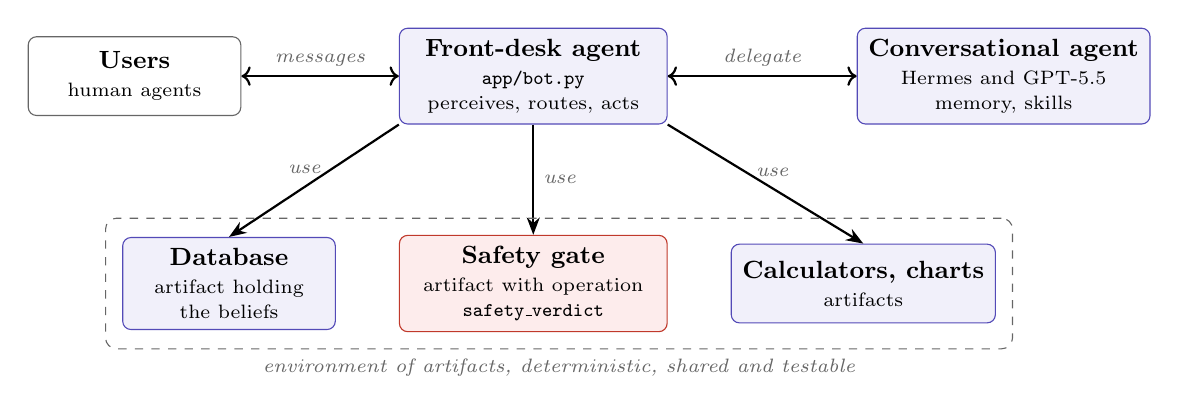
\begin{tikzpicture}[node distance=7mm and 10mm]
  \node[ext,minimum width=27mm] (users) {\textbf{Users}\\[-1pt]\scriptsize human agents};
  \node[box,right=20mm of users,minimum width=34mm] (desk) {\textbf{Front-desk agent}\\[-1pt]\scriptsize \texttt{app/bot.py}\\[-2pt]\scriptsize perceives, routes, acts};
  \node[box,right=24mm of desk,minimum width=33mm] (hermes) {\textbf{Conversational agent}\\[-1pt]\scriptsize Hermes and GPT-5.5\\[-2pt]\scriptsize memory, skills};
  \node[gate,below=14mm of desk,minimum width=34mm] (gate) {\textbf{Safety gate}\\[-1pt]\scriptsize artifact with operation\\[-2pt]\scriptsize \texttt{safety\_verdict}};
  \node[box,left=8mm of gate,minimum width=27mm] (db) {\textbf{Database}\\[-1pt]\scriptsize artifact holding\\[-2pt]\scriptsize the beliefs};
  \node[box,right=8mm of gate,minimum width=33mm] (tools) {\textbf{Calculators, charts}\\[-1pt]\scriptsize artifacts};
  \draw[arr,<->] (users) -- node[lbl,above]{messages} (desk);
  \draw[arr,<->] (desk) -- node[lbl,above]{delegate} (hermes);
  \draw[arr] (desk) -- node[lbl,right]{use} (gate);
  \draw[arr] (desk.south west) -- node[lbl,left,pos=0.4]{use} (db.north);
  \draw[arr] (desk.south east) -- node[lbl,right,pos=0.4]{use} (tools.north);
  \node[draw=muted,dashed,rounded corners,fit=(db)(gate)(tools),inner sep=6pt,
        label={[lbl]below:{environment of artifacts, deterministic, shared and testable}}] {};
\end{tikzpicture}
\caption{NutriGent seen as a multi-agent system. Agents decide and artifacts are used. The
conversational agent never decides food safety and can only reach the user through the front desk.}
\label{fig:mas}
\end{figure}

% =========================================================================
\section{Employed Technologies}\label{sec:tech}

\paragraph{Python 3.12.} The whole engine is written in Python using mostly the standard library, with
\texttt{urllib} for HTTP, \texttt{sqlite3} for storage, and \texttt{json}, \texttt{threading} and
\texttt{subprocess}. Application code is about 1{,}900 lines and tests about 1{,}100 lines.

\paragraph{Telegram Bot API as the interface~\cite{telegrambotapi}.} Telegram is only the user
interface, and the engine does not depend on it. The bot uses \emph{long polling}
(\texttt{getUpdates}), so the server needs no public port, and three kinds of interface elements, a
persistent reply keyboard under the input field, inline keyboards attached to messages, and the
slash-command menu.

\paragraph{SQLite.} One database file holds all state in 15 tables. Migrations are idempotent and run
at start-up, so an existing database is upgraded in place.

\paragraph{Matplotlib.} Verdict cards, dashboards and charts are rendered as PNG images with the
non-interactive Agg backend and sent as photos.

\paragraph{Hermes Agent~\cite{hermesagent} and GPT-5.5.} Hermes Agent is an open-source agent runtime
with tools, persistent memory, skills and a scheduler. It runs on the server under its own profile
(persona, memory and 947 messages of history restored from a backup) and uses OpenAI's GPT-5.5 model.
The engine calls it as a command-line program in one-shot mode (Section~\ref{sec:bridge}). An optional
OpenAI API key enables direct vision extraction and meal planning in \texttt{app/llm.py}. Without it,
the system uses built-in sample answers so that every flow can run offline.

\paragraph{pip and make.} Build automation uses pip. The file \texttt{pyproject.toml} declares the
project and reads its dependencies from \texttt{requirements.txt}, so \texttt{pip install -e .}
prepares an environment. A small \texttt{Makefile} wraps the common tasks (\texttt{install},
\texttt{test}, \texttt{e2e}, \texttt{run}, \texttt{report}).

\paragraph{systemd and Ubuntu.} The pilot runs as a hardened systemd service on Ubuntu 24.04.

\paragraph{LaTeX.} This report is written in LaTeX and built with Tectonic (\texttt{make report}).

% =========================================================================
\section{The System}\label{sec:system}

\subsection{Project folder structure}

Figure~\ref{fig:tree} shows the repository. Runtime code is split between \texttt{app/}, which adapts
the engine to the messaging interface, and \texttt{shared/}, which holds the engine and its artifacts
and is independent of the interface.

\begin{figure}[H]
\centering
\begin{minipage}{0.9\textwidth}
\dirtree{%
.1 nutrigent/.
.2 app/.
.3 bot.py\DTcomment{polling loop and router, the front-desk agent}.
.3 onboarding.py\DTcomment{sign-up state machine}.
.3 handlers.py\DTcomment{one function per user action}.
.3 hermes\_bridge.py\DTcomment{calls the Hermes agent for chat and estimates}.
.3 pending.py\DTcomment{what the user's next typed message means}.
.3 llm.py\DTcomment{OpenAI adapter for extraction and planning}.
.2 shared/.
.3 safety\_gate.py\DTcomment{deterministic verdict engine, an artifact}.
.3 nutrition.py\DTcomment{Mifflin-St Jeor targets and macro split}.
.3 visuals.py, charts.py, reporting.py\DTcomment{PNG cards and charts}.
.3 telegram\_io.py, telegram\_menu.py\DTcomment{interface client and keyboards}.
.3 db.py, schema.sql, allergen\_seed.sql\DTcomment{storage, schema, 145 synonyms}.
.3 prompts/\DTcomment{extraction and planning prompts}.
.2 skills/\DTcomment{15 Hermes skills, one SKILL.md each}.
.2 tests/\DTcomment{unit suites, end-to-end test, fixtures}.
.2 deploy/\DTcomment{systemd unit and Hermes wrapper}.
.2 report/\DTcomment{this report with its figures}.
.2 AGENT\_PROMPT.md\DTcomment{persona and rules for the Hermes agent}.
.2 README.md, FEATURES.md\DTcomment{documentation}.
.2 pyproject.toml, requirements.txt, Makefile\DTcomment{build automation}.
.2 .gitignore, .env.example\DTcomment{repository hygiene and configuration}.
}
\end{minipage}
\caption{The project folder structure.}
\label{fig:tree}
\end{figure}

\subsection{Architecture}

Figure~\ref{fig:arch} shows the deployed architecture. Users talk to the system through the Telegram
interface. The module \texttt{app/bot.py} fetches incoming messages and routes each one. Commands,
buttons and photos go to the deterministic handlers, and open conversation goes to Hermes through
\texttt{app/hermes\_bridge.py}. Handlers read and write the database, call the safety gate and the
calculators, and send image cards. The language model appears in two places only, as the extraction
step of a safety check (via \texttt{app/llm.py}) and as the conversational agent. Neither can issue a
verdict.

\begin{figure}[H]
\centering
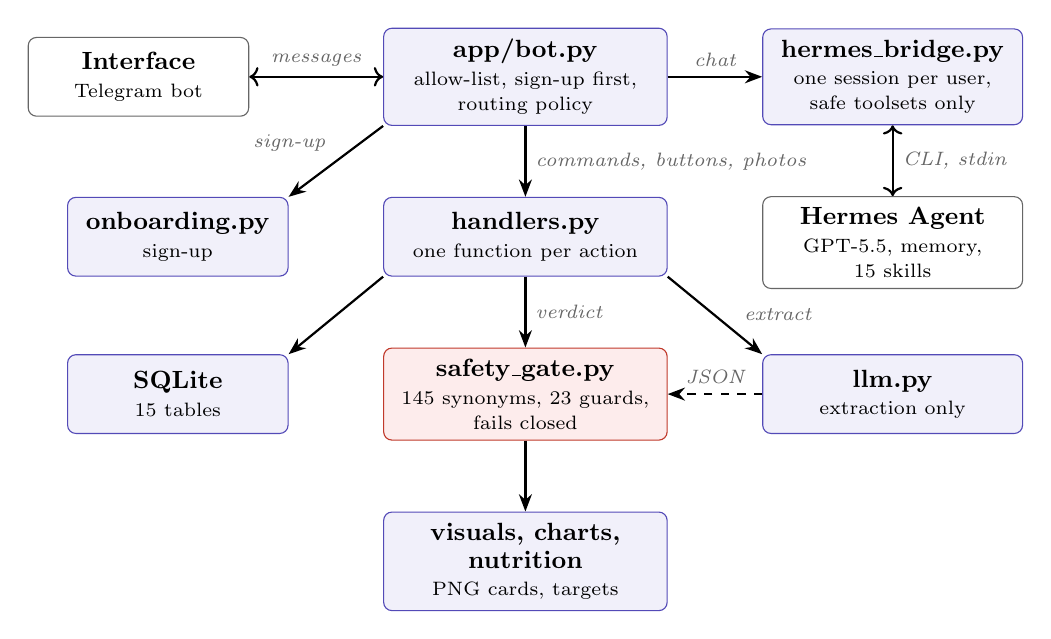
\begin{tikzpicture}[node distance=8mm and 9mm]
  \node[ext,minimum width=28mm] (tg) {\textbf{Interface}\\[-1pt]\scriptsize Telegram bot};
  \node[box,right=17mm of tg,minimum width=36mm] (bot) {\textbf{app/bot.py}\\[-1pt]\scriptsize allow-list, sign-up first,\\[-2pt]\scriptsize routing policy};
  \node[box,right=12mm of bot,minimum width=33mm] (bridge) {\textbf{hermes\_bridge.py}\\[-1pt]\scriptsize one session per user,\\[-2pt]\scriptsize safe toolsets only};
  \node[ext,below=9mm of bridge,minimum width=33mm] (hermes) {\textbf{Hermes Agent}\\[-1pt]\scriptsize GPT-5.5, memory,\\[-2pt]\scriptsize 15 skills};
  \node[box,below=9mm of bot,minimum width=36mm] (handlers) {\textbf{handlers.py}\\[-1pt]\scriptsize one function per action};
  \node[box,left=12mm of handlers,minimum width=28mm] (onb) {\textbf{onboarding.py}\\[-1pt]\scriptsize sign-up};
  \node[gate,below=9mm of handlers,minimum width=36mm] (gate) {\textbf{safety\_gate.py}\\[-1pt]\scriptsize 145 synonyms, 23 guards,\\[-2pt]\scriptsize fails closed};
  \node[box,left=12mm of gate,minimum width=28mm] (db) {\textbf{SQLite}\\[-1pt]\scriptsize 15 tables};
  \node[box,right=12mm of gate,minimum width=33mm] (llm) {\textbf{llm.py}\\[-1pt]\scriptsize extraction only};
  \node[box,below=9mm of gate,minimum width=36mm] (vis) {\textbf{visuals, charts,}\\[-1pt]\textbf{nutrition}\\[-1pt]\scriptsize PNG cards, targets};
  \draw[arr,<->] (tg) -- node[lbl,above]{messages} (bot);
  \draw[arr] (bot) -- node[lbl,above]{chat} (bridge);
  \draw[arr,<->] (bridge) -- node[lbl,right]{CLI, stdin} (hermes);
  \draw[arr] (bot) -- node[lbl,right]{commands, buttons, photos} (handlers);
  \draw[arr] (bot.south west) -- node[lbl,above left]{sign-up} (onb.north east);
  \draw[arr] (handlers) -- node[lbl,right]{verdict} (gate);
  \draw[arr] (handlers.south west) -- (db.north east);
  \draw[arr] (handlers.south east) -- node[lbl,above right,pos=0.7]{extract} (llm.north west);
  \draw[arr,dashed] (llm) -- node[lbl,above]{JSON} (gate);
  \draw[arr] (gate) -- (vis);
\end{tikzpicture}
\caption{Deployed architecture. The red artifact decides safety, and the language model only proposes.}
\label{fig:arch}
\end{figure}

The architecture follows a layered style with dependency inversion at the edges. The \texttt{shared/}
layer knows nothing about the messaging interface and can be tested in isolation, while \texttt{app/}
adapts it to Telegram. The sending functions (\texttt{send\_text}, \texttt{send\_photo} and so on) are
plain module attributes, so tests replace them with recorders and observe exactly what a user would
receive. The same seam is used for the agent, since \texttt{hermes\_bridge.RUNNER} can be replaced by a
fake Hermes in tests. Replacing Telegram with another interface would only touch \texttt{app/}.

\subsection{Core components}

\paragraph{Front-desk agent (\texttt{app/bot.py}).} An endless loop calls \texttt{getUpdates} with a
long timeout and processes each incoming message. It applies the allow-list
(\texttt{ALLOWED\_TELEGRAM\_IDS}), sends users who are in the middle of sign-up to the current
question, translates button-grid labels such as ``Today'' into commands, and dispatches the message
according to the routing policy of Section~\ref{sec:routing}. Chat requests run in a small thread pool
with two workers, so that a slow agent reply never blocks other users.

\paragraph{Sign-up (\texttt{app/onboarding.py}).} A finite-state machine that interviews new users one
question at a time and stores progress in the \texttt{onboarding\_state} table
(Section~\ref{sec:fsm}).

\paragraph{Handlers (\texttt{app/handlers.py}).} One function per user action. The actions are check a
food, show the dashboards, plan the week, show the shopping list, show tonight's meal, cook, swap or show
a recipe, log a meal or a symptom, the ``too tired'' fallback, the weekly report, the allergy card and
the profile.

\paragraph{Pending input (\texttt{app/pending.py}).} Some buttons ask the user to type something next
(``Type a food name'', ``Type it'', ``Other symptom''). The expected kind of input is stored per user
for 30 minutes, so the next plain message is routed to that action instead of the chat agent.

\paragraph{Agent bridge (\texttt{app/hermes\_bridge.py}).} Runs Hermes as a subprocess, keeps one agent
session per user and returns either an answer or \texttt{None}, never an exception
(Section~\ref{sec:bridge}).

\paragraph{LLM adapter (\texttt{app/llm.py}).} The only module that calls the OpenAI API directly. It
turns a photo or a dish name into a strict JSON \emph{extraction} and produces weekly plans and meal
estimates. When no key is configured it falls back to Hermes for estimates and to fixed sample answers
otherwise.

\paragraph{Safety gate (\texttt{shared/safety\_gate.py}).} The deterministic verdict engine
(Section~\ref{sec:gate}).

\paragraph{Calculators and renderers.} \texttt{nutrition.py} computes targets
(Section~\ref{sec:nutrition}), \texttt{visuals.py} and \texttt{charts.py} render cards and charts, and
\texttt{reporting.py} turns database rows into chart inputs.

\paragraph{Hermes skills (\texttt{skills/}).} Fifteen Markdown procedures that teach the agent the
project's workflows (Table~\ref{tab:skills} in Appendix~\ref{app:skills}).

\subsection{User interface}

Users never need to remember a command. Three interface layers coexist. The first is a persistent grid
of 14 buttons under the input field, labelled without slashes (``Today'', ``Plan'', ``Check''). The
second is inline buttons attached to messages, such as the 12-button main menu, sign-up choices,
per-item shopping buttons, tonight's meal actions and the symptom picker. The third is the classic
slash-command menu. Structured answers are images rendered from real database rows with one colour
language, green for safe or on target, amber for caution or under target, red for unsafe or over
target, purple for the brand and target lines, and grey for ``cannot verify''.
Figures~\ref{fig:verdicts} and~\ref{fig:cards} were produced by the system during the end-to-end test,
for test users with fictional data.

\begin{figure}[H]
\centering
\begin{subfigure}{0.48\textwidth}\centering
  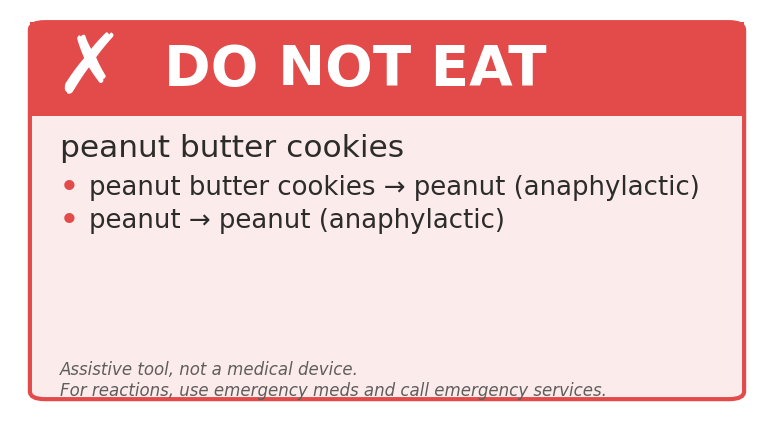
\includegraphics[width=\linewidth]{figures/verdict_unsafe.png}
  \caption{Peanut butter cookies, anaphylactic peanut allergy.}
\end{subfigure}\hfill
\begin{subfigure}{0.48\textwidth}\centering
  
\includegraphics[width=\linewidth]{figures/verdict_caution.png}
  \caption{Photo of a cooked dish, where absence cannot be proven.}
\end{subfigure}
\caption{Verdict cards. Every DO NOT EAT and CAN'T VERIFY card carries emergency guidance.}
\label{fig:verdicts}
\end{figure}

\begin{figure}[H]
\centering
\begin{subfigure}{0.48\textwidth}\centering
  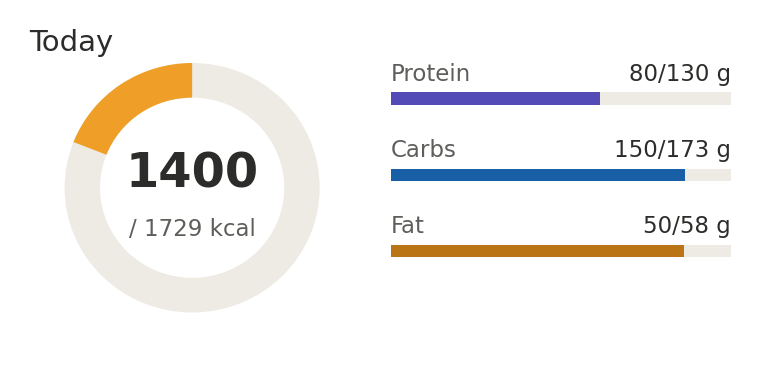
\includegraphics[width=\linewidth]{figures/today.png}
  \caption{Today, with calorie ring and macro bars.}
\end{subfigure}\hfill
\begin{subfigure}{0.48\textwidth}\centering
  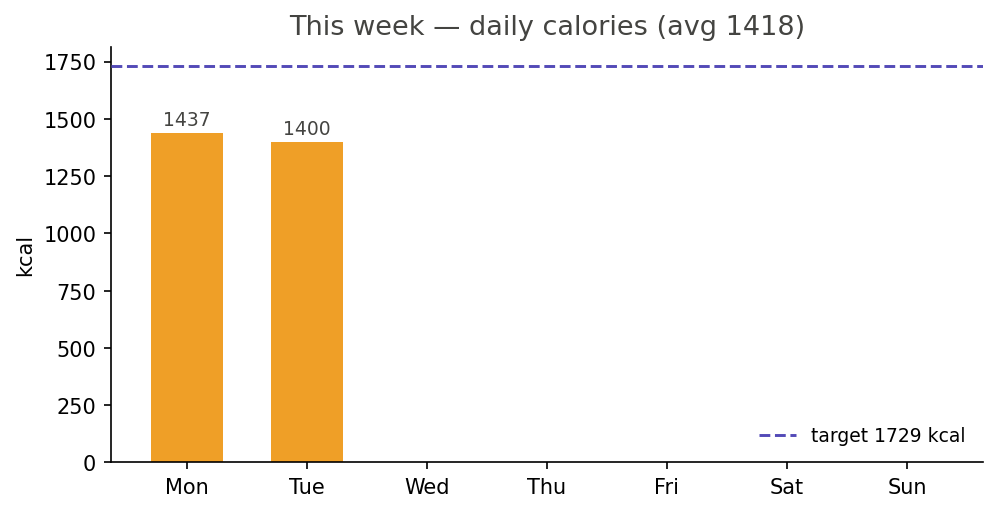
\includegraphics[width=\linewidth]{figures/week.png}
  \caption{Week, daily calories against the target.}
\end{subfigure}\\[6pt]
\begin{subfigure}{0.48\textwidth}\centering
  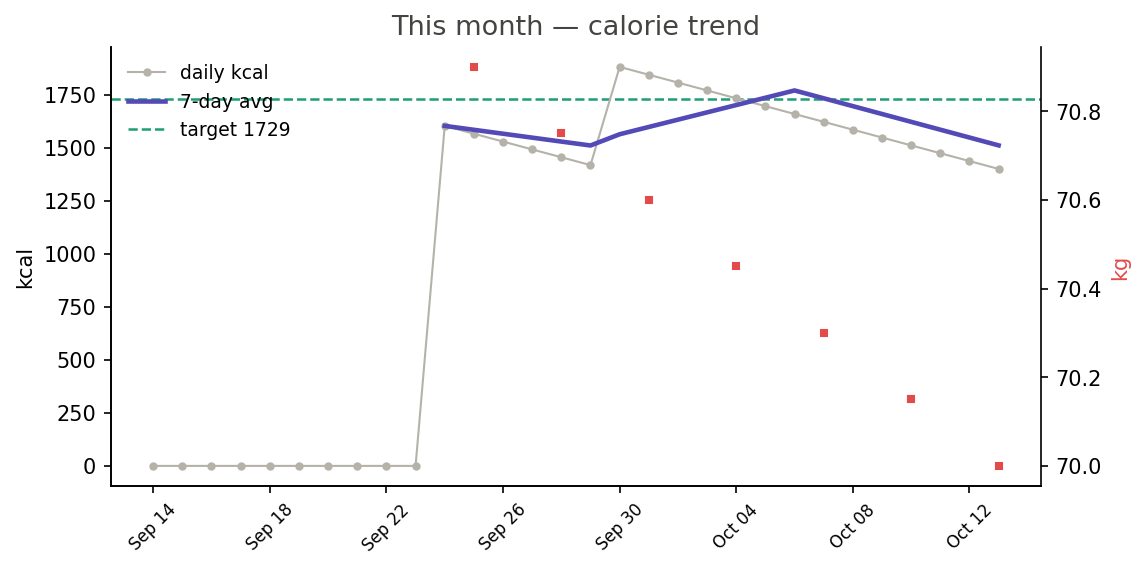
\includegraphics[width=\linewidth]{figures/month.png}
  \caption{Month, 30 days with 7-day average and weight.}
\end{subfigure}\hfill
\begin{subfigure}{0.34\textwidth}\centering
  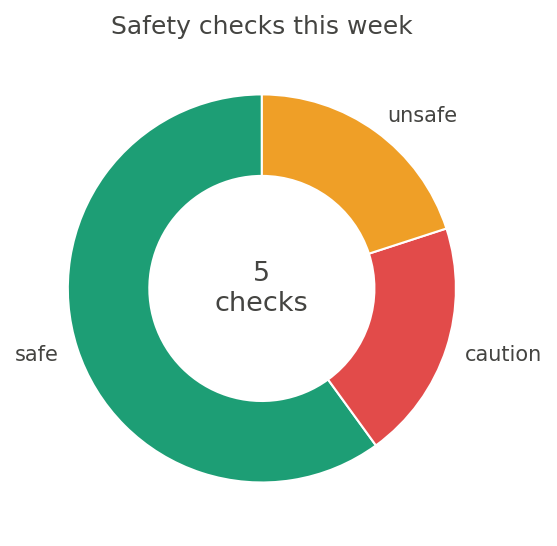
\includegraphics[width=\linewidth]{figures/safety_donut.png}
  \caption{The week's safety checks.}
\end{subfigure}
\caption{Tracking cards.}
\label{fig:cards}
\end{figure}

% =========================================================================
\section{Design and Analysis}\label{sec:design}

\subsection{The deterministic safety gate}\label{sec:gate}

The gate turns an \emph{extraction} and a \emph{profile} into one of five verdicts, namely DO NOT EAT,
CAUTION, LIKELY SAFE, SAFE and CAN'T VERIFY. The extraction is the only thing a language model
contributes. It is a JSON object with the fields of Table~\ref{tab:extraction}.

\begin{table}[H]
\centering\small
\caption{Fields of an extraction, with an example for a chocolate bar label.}
\label{tab:extraction}
\begin{tabularx}{\textwidth}{@{}l Y l@{}}
\toprule
Field & Meaning & Example \\
\midrule
\texttt{image\_type} & ingredient label, prepared food, menu, unreadable or not food & ingredient label \\
\texttt{readability} & how much of a label could be read, from 0 to 1 & 0.95 \\
\texttt{identified\_ingredients} & ingredients that are declared or visible & sugar, whey powder, cocoa \\
\texttt{likely\_hidden\_ingredients} & typical ingredients that are not visible & none \\
\texttt{precautionary\_warnings} & ``may contain'' statements & may contain peanut \\
\bottomrule
\end{tabularx}
\end{table}

\noindent The gate works in four stages.

\paragraph{1. Resolving the user's allergies.} Users write allergies in their own words. The gate maps
them to the 14 canonical allergens of EU Regulation 1169/2011, Annex~II~\cite{eu1169}, which also cover
the nine major allergens of United States law~\cite{faster2021}. They are celery, egg, fish, lupin,
milk, mollusc, mustard, peanut, sesame, shellfish, soy, sulphite, tree nut and wheat. Aliases are
resolved (\emph{dairy} and \emph{lactose} become milk, \emph{gluten} becomes wheat, \emph{seafood}
becomes shellfish, mollusc and fish), plurals are handled, and an ambiguous word maps to \emph{every}
allergen it could mean (\emph{nuts} becomes tree nut and peanut). When two entries map to the same
allergen the strictest severity wins. An allergen without a synonym list, for example kiwi, is matched
by its literal name and can never yield SAFE. Algorithm~\ref{alg:resolve} in Appendix~\ref{app:alg}
gives the procedure.

\paragraph{2. Matching.} Each ingredient is normalised (lower case, punctuation removed) and compared
with 145 synonyms, either as a substring (``whey'' in ``whey powder'') or exactly (E-numbers such as
E220 to E228). Table~\ref{tab:syn} shows a sample.

\begin{table}[H]
\centering\small
\caption{Sample of the synonym table, which has 145 terms for 14 allergens.}
\label{tab:syn}
\begin{tabularx}{\textwidth}{@{}l Y@{}}
\toprule
Allergen & Examples of label terms that trigger it \\
\midrule
milk & whey, casein, caseinate, lactose, lactalbumin, butter, E966, lactitol \\
egg & albumin, albumen, ovalbumin, lysozyme, mayonnaise, E1105 \\
fish & anchovy, Worcestershire sauce, fish sauce, surimi, caviar \\
soy & lecithin, E322, tamari, miso, edamame, natto \\
wheat & gluten, semolina, spelt, durum, bulgur, seitan, farro, kamut, barley, rye, malt \\
sulphite & E220 to E228 (exact match), metabisulphite \\
\bottomrule
\end{tabularx}
\end{table}

\paragraph{3. False-positive guards.} Substring matching alone would raise false alarms, so 23 guards
skip known traps. Examples are coconut, almond, oat, rice and soy milk, cocoa and shea butter, peanut
butter for milk, nutmeg, water chestnut and coconut for tree nuts, buckwheat for wheat, eggplant for
egg, and ``free from'' claims.

\paragraph{4. Policy.} The matches are classified by where they were found (declared ingredients,
likely-hidden ingredients, precautionary warnings), and the policy of Table~\ref{tab:policy} is
applied, strictest rule first.

\begin{table}[H]
\centering\small
\caption{Verdict policy, checked from top to bottom.}
\label{tab:policy}
\begin{tabularx}{\textwidth}{@{}c Y l@{}}
\toprule
\# & Condition & Verdict \\
\midrule
1 & Input unusable, that is not food, unreadable, or a label with readability below 0.85 & CAN'T VERIFY \\
2 & A user allergen is among the declared ingredients & DO NOT EAT \\
3 & A ``may contain'' trace, and the user's severity is severe or anaphylactic & DO NOT EAT \\
4 & A trace or likely-hidden allergen at lower severity & CAUTION \\
5 & The user has an allergen without a synonym list & CAUTION \\
6 & Photo of a cooked dish or of a menu, and a severe or anaphylactic allergy & CAUTION \\
7 & Photo of a cooked dish or of a menu otherwise & LIKELY SAFE \\
8 & Complete, readable ingredient list with no match & SAFE \\
\bottomrule
\end{tabularx}
\end{table}

\paragraph{Properties.} Three properties follow directly from this design and are checked by the tests.
\emph{Determinism} holds because the function reads only its inputs and static tables, so the same
extraction and profile always give the same verdict. \emph{Fail-closed} behaviour holds because every
source of uncertainty (unusable input, unknown allergen, a photo that cannot show the recipe, a menu)
maps to a verdict weaker than SAFE. \emph{Monotonicity in evidence} holds because the policy checks hits
before it ever reaches a SAFE rule, so adding an ingredient can only keep or lower the verdict.

\paragraph{A worked example.} A user with a moderate fish allergy asks about a beef stew whose label
lists ``beef, Worcestershire sauce''. The gate normalises the terms, finds the synonym
``worcestershire'' under fish, checks that no guard applies, and returns DO NOT EAT. The reason shown
to the user names the matched term (Worcestershire sauce), the allergen (fish), the severity (moderate)
and where it was found (the ingredients).

\subsection{Routing policy, or who may answer what}\label{sec:routing}

Because one front-desk agent receives everything, the routing policy is where safety is enforced at the
organisational level. The policy is an ordered list of rules (Algorithm~\ref{alg:route} in
Appendix~\ref{app:alg}), summarised in Figure~\ref{fig:route}. The key rule is that \emph{questions
about food safety never reach the conversational agent}. A photo, a ``can I eat \ldots'' question or a
typed food name after the Check button always goes to the gate. The agent is also told, in the context
of every message, never to judge food safety and to point the user to the Check button.

\begin{figure}[H]
\centering
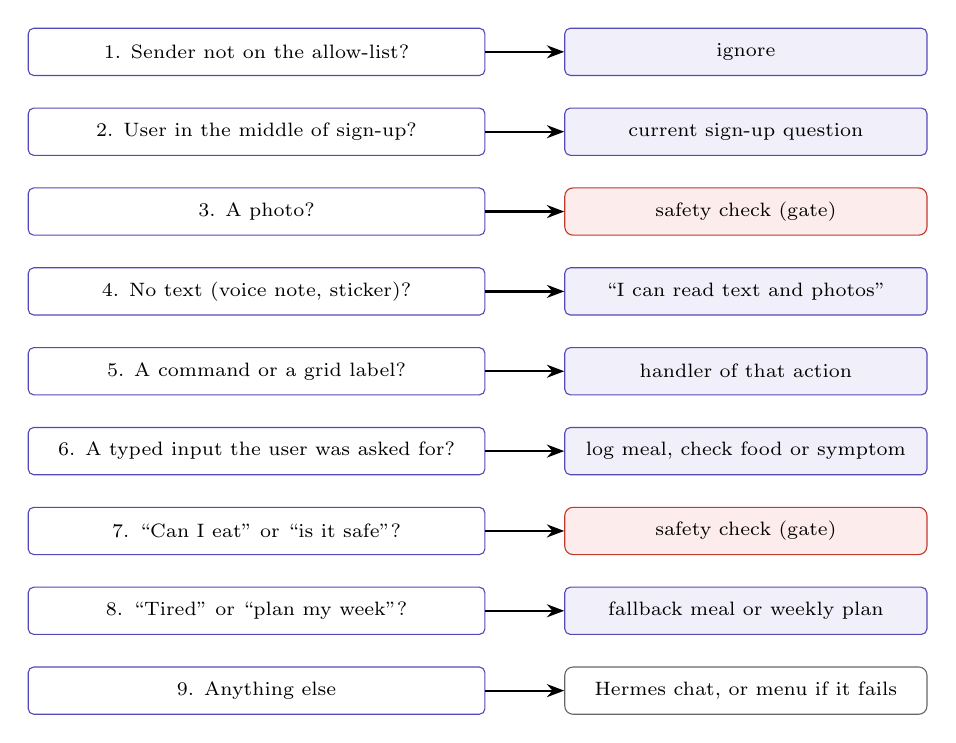
\begin{tikzpicture}[node distance=4mm,
  q/.style={draw=accent,fill=white,rounded corners=2pt,font=\scriptsize,align=left,
            minimum width=58mm,minimum height=6mm,inner sep=3pt},
  a/.style={draw=accent,fill=soft,rounded corners=2pt,font=\scriptsize,align=left,
            minimum width=46mm,minimum height=6mm,inner sep=3pt}]
  \node[q] (r1) {1. Sender not on the allow-list?};
  \node[q,below=of r1] (r2) {2. User in the middle of sign-up?};
  \node[q,below=of r2] (r3) {3. A photo?};
  \node[q,below=of r3] (r4) {4. No text (voice note, sticker)?};
  \node[q,below=of r4] (r5) {5. A command or a grid label?};
  \node[q,below=of r5] (r6) {6. A typed input the user was asked for?};
  \node[q,below=of r6] (r7) {7. ``Can I eat'' or ``is it safe''?};
  \node[q,below=of r7] (r8) {8. ``Tired'' or ``plan my week''?};
  \node[q,below=of r8] (r9) {9. Anything else};
  \node[a,right=10mm of r1] (a1) {ignore};
  \node[a,right=10mm of r2] (a2) {current sign-up question};
  \node[gate,right=10mm of r3,minimum width=46mm,minimum height=6mm,font=\scriptsize,inner sep=3pt] (a3) {safety check (gate)};
  \node[a,right=10mm of r4] (a4) {``I can read text and photos''};
  \node[a,right=10mm of r5] (a5) {handler of that action};
  \node[a,right=10mm of r6] (a6) {log meal, check food or symptom};
  \node[gate,right=10mm of r7,minimum width=46mm,minimum height=6mm,font=\scriptsize,inner sep=3pt] (a7) {safety check (gate)};
  \node[a,right=10mm of r8] (a8) {fallback meal or weekly plan};
  \node[ext,right=10mm of r9,minimum width=46mm,minimum height=6mm,font=\scriptsize,inner sep=3pt,align=left] (a9) {Hermes chat, or menu if it fails};
  \foreach \i in {1,...,9} {\draw[arr] (r\i) -- (a\i);}
\end{tikzpicture}
\caption{The routing policy of the front-desk agent, where the first matching rule wins. Red boxes
mark the cases decided by the gate artifact.}
\label{fig:route}
\end{figure}

\subsection{The agent bridge}\label{sec:bridge}

The bridge connects the front-desk agent to Hermes without giving up control. Its design responds to
four concerns.

\paragraph{Isolation of user text.} The user's message is passed on standard input
(\texttt{--query-file -}), never through a shell or the argument list, so it cannot be interpreted as a
command-line option or shell syntax.

\paragraph{Least privilege.} Hermes is started with only five toolsets, \texttt{memory},
\texttt{session\_search}, \texttt{skills}, \texttt{web} and \texttt{vision}. Terminal, file, code
execution, browser and computer-use tools are not available, so a prompt-injection
attempt~\cite{greshake2023} by a user cannot make the agent run commands on the server. A test on the
server confirmed that the agent refuses shell requests. The number of reasoning turns is capped at six.

\paragraph{Per-user memory.} Each user has one Hermes session, stored in the \texttt{hermes\_sessions}
table and resumed on every message, so the conversation has continuity. If a stored session cannot be
resumed, the bridge forgets it and starts a fresh one (Algorithm~\ref{alg:ask}). Every message carries
a short context with the user's profile (allergies with severity, diet, goal) and three rules. The
agent must reply in the user's language and in plain text, must never judge food safety, and must
remember that it is not a medical device.

\paragraph{Graceful degradation.} A missing binary, a non-zero exit code, a timeout (120\,s for chat,
60\,s for estimates) or an empty answer all yield \texttt{None}. The front desk then replies ``Sorry, I
couldn't answer that right now'' with the main menu, so the user is never left in silence. While the
agent thinks, the bot repeats the ``typing'' indicator every four seconds.

The same bridge provides \emph{meal estimates}. When the user logs ``chicken salad with rice'', Hermes is
asked for a JSON object with kcal and macros. The answer is \emph{validated} before use (kcal strictly
between 0 and 5000, each macro between 0 and 500\,g), and otherwise the meal is stored without calories
and the user is told. This is again \emph{propose and dispose}, since the model suggests a number and
code decides whether it is plausible.

\subsection{Sign-up as a finite-state machine}\label{sec:fsm}

The first version of sign-up had no memory of which question had been asked, which produced a loop in
pilot testing (Section~\ref{sec:defects}). It was redesigned as an explicit state machine
(Figure~\ref{fig:fsm}). The state, made of the current step and the answers so far, is stored in the
database before the next question is sent, so a restart never loses progress and an answered question
is never asked again. Each step validates its input. Allergy taps toggle a selection and typed allergies
are comma-separated. Numbers are checked against human ranges (age 13 to 100, height 120 to 230\,cm,
weight 30 to 300\,kg), and invalid input re-asks the same question. Commands and grid buttons pressed
during sign-up re-ask the current question instead of starting another action, while \texttt{/start}
always restarts.

\begin{figure}[H]
\centering
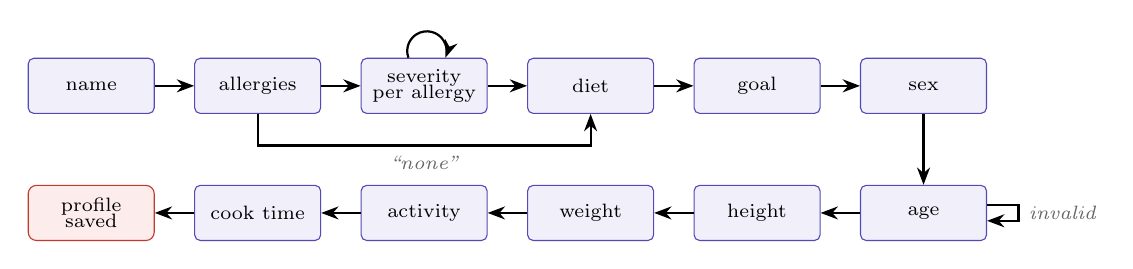
\begin{tikzpicture}[
  st/.style={draw=accent,fill=soft,rounded corners=2pt,font=\scriptsize,minimum width=16mm,
             minimum height=7mm,align=center},
  node distance=5mm]
  \node[st] (s1) {name};
  \node[st,right=of s1] (s2) {allergies};
  \node[st,right=of s2] (s3) {severity\\[-2pt]per allergy};
  \node[st,right=of s3] (s4) {diet};
  \node[st,right=of s4] (s5) {goal};
  \node[st,right=of s5] (s6) {sex};
  \node[st,below=9mm of s6] (s7) {age};
  \node[st,left=of s7] (s8) {height};
  \node[st,left=of s8] (s9) {weight};
  \node[st,left=of s9] (s10) {activity};
  \node[st,left=of s10] (s11) {cook time};
  \node[gate,left=of s11,minimum width=16mm,minimum height=7mm,font=\scriptsize] (done) {profile\\[-2pt]saved};
  \foreach \a/\b in {s1/s2,s2/s3,s3/s4,s4/s5,s5/s6,s6/s7,s7/s8,s8/s9,s9/s10,s10/s11,s11/done}
    {\draw[arr] (\a) -- (\b);}
  \draw[arr] (s3.north) ++(-2mm,0) arc[start angle=200,end angle=-20,radius=2.5mm];
  \draw[arr] (s2.south) -- ++(0,-4mm) -| node[lbl,below,pos=0.25]{``none''} (s4.south);
  \draw[arr] (s7.east) ++(0,1mm) -- ++(4mm,0) |- node[lbl,right,pos=0.25]{invalid} ($(s7.east)+(0,-1mm)$);
\end{tikzpicture}
\caption{The sign-up state machine with eleven questions, mostly answered with buttons. Severity is
asked once per allergy, ``none'' skips it, and invalid numbers stay in the same state.}
\label{fig:fsm}
\end{figure}

\subsection{Nutrition model}\label{sec:nutrition}

Daily energy targets use the Mifflin-St Jeor equation~\cite{mifflin1990} for basal metabolic rate
(BMR), multiplied by an activity factor to obtain total daily energy expenditure (TDEE), then adjusted
for the goal.
\begin{align}
\mathrm{BMR} &= 10\,w + 6.25\,h - 5\,a + s, \qquad s = \begin{cases}+5 & \text{men}\\ -161 & \text{women}\end{cases}\\
\mathrm{TDEE} &= \mathrm{BMR}\cdot f, \qquad f \in \{1.2,\ 1.375,\ 1.55,\ 1.725,\ 1.9\}\\
\mathrm{target} &= \mathrm{TDEE}\cdot g, \qquad g = 0.80\ \text{(lose)},\ 1.00\ \text{(maintain)},\ 1.12\ \text{(gain)}
\end{align}
Here $w$ is weight in kg, $h$ height in cm and $a$ age in years, and the five factors correspond to
sedentary, light, moderate, active and athlete. Macronutrients are split into 30\,\% protein, 40\,\%
carbohydrate and 30\,\% fat, at 4, 4 and 9\,kcal per gram. For example, a 29-year-old woman, 165\,cm and
60\,kg, moderately active and wanting to lose weight, gets a BMR of 1{,}325, a TDEE of 2{,}054 and a
target of 1{,}643\,kcal (123\,g protein, 164\,g carbohydrate, 55\,g fat). Both this and a second example
appear in the automated tests. The 20\,\% deficit and 12\,\% surplus are conservative defaults.

\subsection{Data model}

All state lives in one SQLite file, which keeps deployment simple and data on the operator's server
(Table~\ref{tab:schema}).

\begin{table}[H]
\centering\small
\caption{Database schema (\texttt{shared/schema.sql}).}
\label{tab:schema}
\begin{tabularx}{\textwidth}{@{}l Y@{}}
\toprule
Table & Purpose \\
\midrule
users & Interface identity, name, time zone, locale \\
dietary\_profiles & Allergies with severity, diet, goal, calorie and macro targets, cooking time, budget,
  eating window, health flags \\
onboarding\_state & Current sign-up step and answers so far \\
hermes\_sessions & The agent session of each user \\
pending\_input & What the user's next typed message means, with a 30-minute expiry \\
allergen\_synonyms & 145 label terms mapped to 14 canonical allergens (contains or exact) \\
synonym\_exceptions & 23 false-positive guards \\
pantry & Ingredients at home, quantity, unit, expiry date \\
recipes & Generated or imported recipes with macros and the gate's screening result \\
meal\_schedule & Planned meals per day and their status (planned, cooked, skipped, swapped) \\
shopping\_list\_items & Weekly list with missing quantity, store section and status \\
food\_log & Everything eaten or checked, with source, verdict, flagged allergens and macros \\
preference\_events & Accepted, swapped, skipped, loved or hated recipes \\
weight\_log, symptom\_log & Weight over time, and symptoms with severity \\
\bottomrule
\end{tabularx}
\end{table}

% =========================================================================
\section{Workflows}\label{sec:workflows}

\subsection{Life of a message}

Figure~\ref{fig:seq} follows a free-text message and a safety question through the system. The two
paths differ in who is allowed to answer, the agent for conversation and the gate for safety.

\begin{figure}[H]
\centering
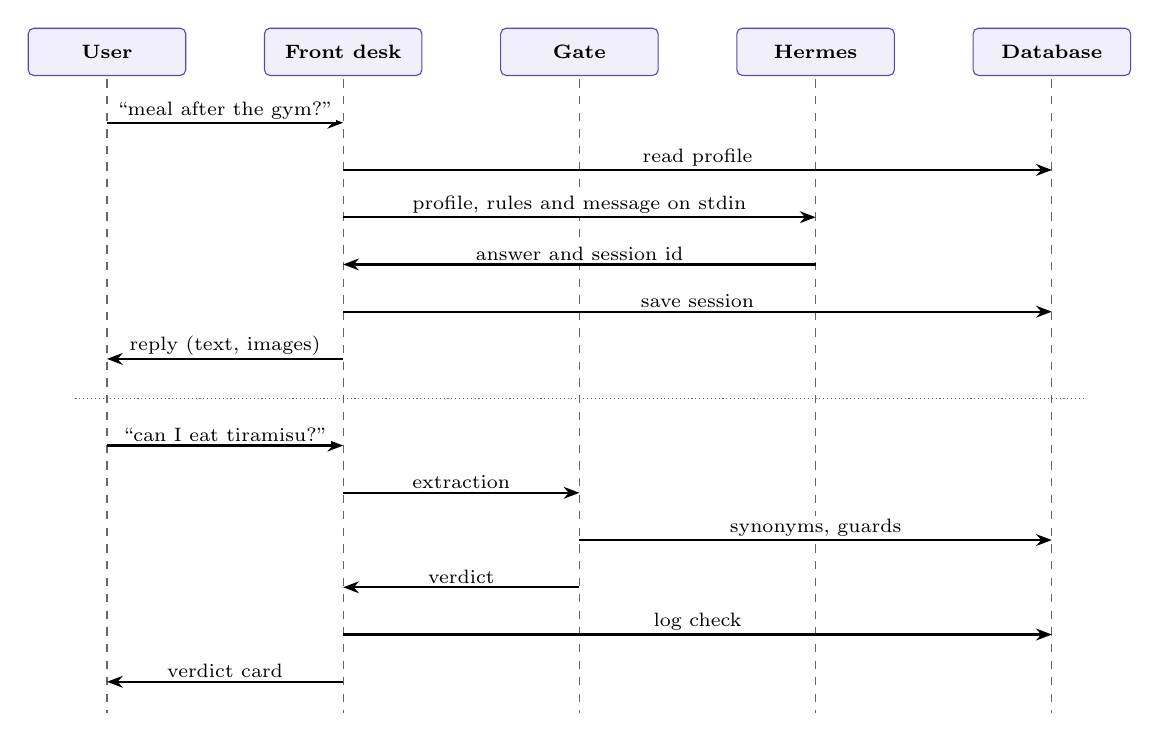
\begin{tikzpicture}[
  ll/.style={draw=muted,dashed},
  hd/.style={draw=accent,fill=soft,rounded corners=2pt,font=\scriptsize\bfseries,minimum width=20mm,
             minimum height=6mm},
  msg/.style={-{Stealth[length=2mm]},thick},
  t/.style={font=\scriptsize,fill=white,inner sep=1pt}]
  \foreach \x/\n/\l in {0/u/User,3/b/Front desk,6/g/Gate,9/h/Hermes,12/d/Database} {
    \node[hd] (\n) at (\x,0) {\l};
    \draw[ll] (\x,-0.35) -- (\x,-8.4);
  }
  \draw[msg] (0,-0.9) -- node[t,above]{``meal after the gym?''} (3,-0.9);
  \draw[msg] (3,-1.5) -- node[t,above]{read profile} (12,-1.5);
  \draw[msg] (3,-2.1) -- node[t,above]{profile, rules and message on stdin} (9,-2.1);
  \draw[msg] (9,-2.7) -- node[t,above]{answer and session id} (3,-2.7);
  \draw[msg] (3,-3.3) -- node[t,above]{save session} (12,-3.3);
  \draw[msg] (3,-3.9) -- node[t,above]{reply (text, images)} (0,-3.9);
  \draw[densely dotted,muted] (-0.4,-4.4) -- (12.4,-4.4);
  \draw[msg] (0,-5.0) -- node[t,above]{``can I eat tiramisu?''} (3,-5.0);
  \draw[msg] (3,-5.6) -- node[t,above]{extraction} (6,-5.6);
  \draw[msg] (6,-6.2) -- node[t,above]{synonyms, guards} (12,-6.2);
  \draw[msg] (6,-6.8) -- node[t,above]{verdict} (3,-6.8);
  \draw[msg] (3,-7.4) -- node[t,above]{log check} (12,-7.4);
  \draw[msg] (3,-8.0) -- node[t,above]{verdict card} (0,-8.0);
\end{tikzpicture}
\caption{Two messages through the system. In the upper part, open conversation goes to the agent with
the user's profile as context. In the lower part, a safety question never reaches the agent, and the
extraction is the JSON proposed by the language model.}
\label{fig:seq}
\end{figure}

\subsection{Food safety check}

The user sends a photo, taps Check and types a dish name, or simply asks ``can I eat \ldots?''. The
input is turned into an extraction. Photos go through vision, and for a dish name the model lists
typical and likely-hidden ingredients (for tiramisu these are mascarpone, eggs, ladyfingers, cream and
coffee). The gate returns a verdict, the system sends the verdict card with the textual reasons, and the
check is logged in \texttt{food\_log}, which feeds the weekly safety chart. The ``Scan a menu'' button
routes the next photo through the same path, and a menu, like a photo of a cooked dish, can never be
called SAFE.

\subsection{Weekly plan, tonight's meal and shopping}

The plan action sends the profile and pantry to the planner model, which returns seven days of recipes.
The plan is \emph{not trusted}, so every recipe is re-screened by the gate before it enters the
schedule. Because a recipe's ingredient list is complete, it is screened like a label, and a recipe that
hits an allergen is marked ``needs regeneration''. The shopping list is computed as \emph{ingredients
required minus pantry stock}, with quantities, grouped by store section. ``Tonight'' shows the planned
meal with three actions. \emph{Cooking it} marks it cooked and logs its macros, \emph{Swap} exchanges it
with the next planned meal, and \emph{Show recipe} sends ingredients and steps. Each shopping item has
``bought'' and ``not available'' buttons, and the system checks that the item belongs to the user who
taps it.

\begin{figure}[H]
\centering
\begin{subfigure}{0.44\textwidth}\centering
  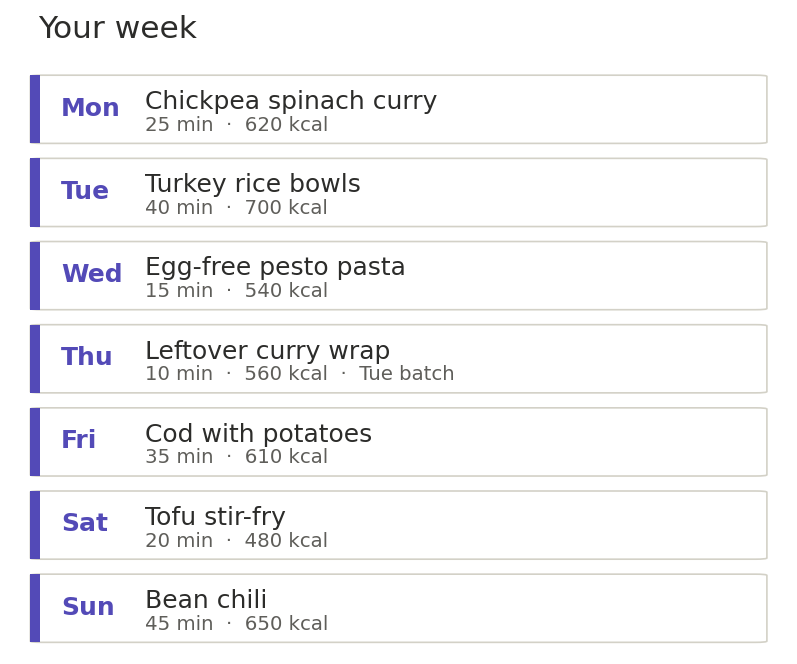
\includegraphics[width=\linewidth]{figures/plan.png}
  \caption{Plan card for a user with an anaphylactic peanut allergy.}
\end{subfigure}\hfill
\begin{subfigure}{0.52\textwidth}\centering
  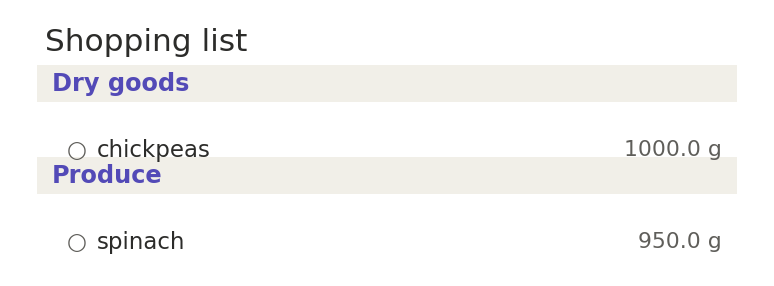
\includegraphics[width=\linewidth]{figures/shopping.png}
  \caption{Shopping list grouped by store section.}\vspace{6pt}
  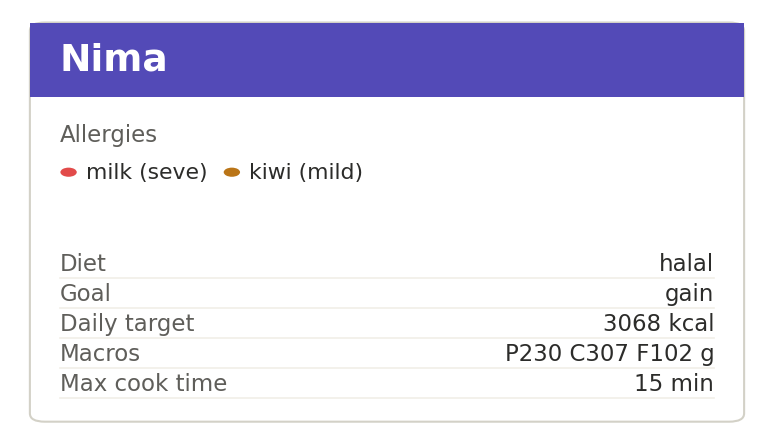
\includegraphics[width=\linewidth]{figures/profile.png}
  \caption{Profile card created by the sign-up.}
\end{subfigure}
\caption{Planning, shopping and profile cards.}
\label{fig:plan}
\end{figure}

\subsection{Logging and tracking}

``Log'' offers three ways to record a meal. ``Type it'' waits for a description, asks the agent for an
estimate (validated as described in Section~\ref{sec:bridge}) and stores a \texttt{food\_log} row.
Photo and voice logging are on the roadmap and say so. ``Symptom'' offers a picker (bloating, low
energy, headache, skin, other) and stores the symptom with a timestamp, the raw material for the planned
food-symptom correlation. ``Today'', ``Week'', ``Month'' and ``Report'' render the cards of
Figure~\ref{fig:cards} from the logs.

% =========================================================================
\section{Development Process}\label{sec:process}

\subsection{Method}

Development followed a \emph{test-first} discipline~\cite{beck2002}. Every behaviour change started
with an automated test, which was run and seen to fail for the expected reason before the code was
changed, and the whole suite was run again before each deployment. A \emph{model-first} step preceded
the code wherever the behaviour was non-trivial. The verdict policy was written as a table
(Table~\ref{tab:policy}), the sign-up as a state machine (Figure~\ref{fig:fsm}) and the routing as an
ordered rule list (Figure~\ref{fig:route}) before being implemented.

The repository follows a simplified GitLab flow, in which \texttt{main} is always deployable and each
change is a focused commit made only after the suites pass locally. The release procedure is to run
all suites locally, copy the committed tree to the server, run all suites on the server, restart the
service and read the logs. The repository is kept clean by a \texttt{.gitignore} that excludes secrets
(\texttt{.env}), databases (which contain health data), caches, virtual environments, build output,
LaTeX output, IDE configuration and operating-system files. No binaries other than the report figures
and one test photo are tracked.

\subsection{Defects found and fixed}\label{sec:defects}

Testing against realistic inputs uncovered several defects, some of them safety-relevant.
Table~\ref{tab:defects} lists them, and each fix is protected by a regression test.

\begin{table}[H]
\centering\small
\caption{Defects found during the project. All are covered by regression tests.}
\label{tab:defects}
\begin{tabularx}{\textwidth}{@{}l Y Y@{}}
\toprule
Defect & Effect & Fix \\
\midrule
Fail-open allergy names & A user who wrote ``dairy'', ``peanuts'', ``gluten'' or ``nuts'' matched nothing,
  so every food was SAFE, a direct violation of G1. & Alias and plural resolution, ambiguous words mapped
  to all candidates, unknown allergens matched literally and capped at CAUTION. \\
Sign-up loop & Every message from a new user produced the same welcome and ``what should I call you?''. &
  Sign-up rebuilt as a persisted state machine. \\
Menu photo called SAFE & A menu without a visible allergen word returned SAFE. & Menus treated like cooked
  dishes (policy rules 6 and 7). \\
Logging marked dinner cooked & Logging any snack marked tonight's planned meal as cooked. & Logging no longer
  touches the schedule, only ``Cooking it'' does. \\
Rejected replies & ``mac \& cheese'' made the interface reject the reply because of HTML parsing. &
  Messages are sent as plain text. \\
Every planned meal flagged & Recipes were screened as photos of cooked dishes, so for severe allergies every
  meal was ``needs regeneration''. & Recipes screened as complete ingredient lists. \\
Text off the card & Long verdict reasons ran past the card edge. & Reasons wrap without splitting words. \\
13 silent buttons & Check, log, symptom and tonight sub-buttons had no handler. & Every button wired, typed
  follow-ups routed by \texttt{pending.py}. \\
Open agent gateway & On the previous server the agent, which can run shell commands, accepted any user and
  ran as root. & Unprivileged user, agent gateway off, allow-list, safe toolsets only. \\
\bottomrule
\end{tabularx}
\end{table}

The fail-open defect deserves a comment because it illustrates the value of the artifact design. The
defect was in the gate, not in the model. Because the gate is deterministic, a table of before and after
cases (Table~\ref{tab:failopen}) could be turned directly into tests, and the fix could be proven
complete for every listed case.

\begin{table}[H]
\centering\small
\caption{Behaviour of the gate before and after the fail-open fix. Each row is a test.}
\label{tab:failopen}
\begin{tabularx}{\textwidth}{@{}l Y l l@{}}
\toprule
User wrote & Label contains & Before & After \\
\midrule
dairy & milk powder & SAFE & DO NOT EAT \\
lactose & whey & SAFE & DO NOT EAT \\
Peanuts & peanut butter & SAFE & DO NOT EAT \\
gluten & wheat flour & SAFE & DO NOT EAT \\
nuts & almonds, or peanut oil & SAFE & DO NOT EAT \\
kiwi (no synonym list) & kiwi fruit, or water and salt & SAFE, SAFE & DO NOT EAT, CAUTION \\
egg & eggplant & DO NOT EAT (false alarm) & SAFE \\
\bottomrule
\end{tabularx}
\end{table}

% =========================================================================
\section{Results}\label{sec:results}

\subsection{Automated tests}

Table~\ref{tab:tests} lists the suites, and \texttt{make test} runs them all. All 45 unit tests and 23
safety fixtures pass (68 checks), on macOS and on the server.

\begin{table}[H]
\centering\small
\caption{Automated test suites.}
\label{tab:tests}
\begin{tabularx}{\textwidth}{@{}l Y r@{}}
\toprule
Suite & What it checks & Result \\
\midrule
test\_safety\_gate & Direct and hidden allergens, traces by severity, unreadable labels, cooked dishes and
  menus, false-positive guards, E-numbers, typed allergy names, unknown allergens & 23 of 23 \\
test\_chat\_and\_buttons & Free chat reaches the agent with the profile, food questions stay with the gate,
  agent failure falls back to the menu, every button, plan screening, card text wrapping, plain text & 19 of 19 \\
test\_hermes\_bridge & Output parsing, per-user sessions, stale-session retry, timeouts, missing binary,
  estimate validation (with a fake Hermes) & 9 of 9 \\
test\_onboarding\_flow & Full sign-up, no loop, bad numbers re-asked, no-allergy path, commands during
  sign-up, returning user & 6 of 6 \\
test\_reply\_keyboard & Grid labels without slashes, persistence, every label runs its command & 5 of 5 \\
test\_access & Allow-list and ownership of shopping items & 4 of 4 \\
test\_onboarding\_buttons & Sign-up button layouts and callback formats & 2 of 2 \\
test\_bot\_flow & Simulated messages through router, handlers and image rendering & runs \\
\bottomrule
\end{tabularx}
\end{table}

\subsection{End-to-end test against a simulated messaging API}

Unit tests replace the network with recorders, so they cannot show what a user actually experiences.
A fake Telegram Bot API was therefore written (\texttt{tests/e2e\_fake\_telegram.py}). It is a small
HTTP server on the local machine implementing \texttt{getUpdates}, \texttt{sendMessage},
\texttt{sendPhoto}, \texttt{sendChatAction}, \texttt{getFile} and \texttt{answerCallbackQuery}. Like the
real service, it rejects messages that break the HTML rules and photos that are not valid images. The
\emph{unmodified} polling loop of \texttt{bot.py} is pointed at it and driven through 80 scripted
actions. They include 19 commands (one deliberately unknown), 29 button taps, two photos, eight
free-text messages including Persian and the characters ``\&'' and ``<'', a voice note, and the
complete 21-step session of a brand-new user. The run takes about 20 seconds and peaks at about
120\,MB of memory.

Table~\ref{tab:e2e} compares the run before and after the work on the core flows. The final run gets a
correct reply to every action, with identical results on the laptop and on the server.

\begin{table}[H]
\centering\small
\caption{End-to-end results, before and after the core-flows phase.}
\label{tab:e2e}
\begin{tabular}{@{}lrr@{}}
\toprule
Outcome & Before & After \\
\midrule
Correct reply & 66 & 80 \\
No reply (buttons without a handler) & 13 & 0 \\
Rejected by the interface (``\&'' in a reply) & 1 & 0 \\
\midrule
Total actions & 80 & 80 \\
\bottomrule
\end{tabular}
\end{table}

A paraphrased excerpt of the new user's session shows the sign-up behaving as designed, including a
grid button pressed during sign-up and an invalid age (Table~\ref{tab:transcript}).

\begin{table}[H]
\centering\small
\caption{Paraphrased excerpt of the sign-up session in the end-to-end run.}
\label{tab:transcript}
\begin{tabularx}{\textwidth}{@{}p{4.3cm} Y@{}}
\toprule
User sends & NutriGent replies \\
\midrule
/start & Greets the user as their diet and allergy assistant and asks what to call them \\
Nima & ``Nice to meet you, Nima!'' and asks about food allergies \\
{[taps Milk]}, types ``kiwi'' & Shows the selection, first milk, then milk and kiwi, and offers Done \\
{[taps the Today grid button]} & ``Let's finish setting you up first.'' and repeats the question \\
{[Done]}, {[Severe]}, {[Mild]} & Asks the severity of each allergy, then the diet \\
abc (as age) & ``Please send a number between 13 and 100.'' and repeats the question \\
\ldots{} {[15 min]} & Sends the profile card and says the user is set \\
/today & Sends the dashboard with 0 of 3068 kcal \\
/start & ``Welcome back, Nima!'' \\
check milk chocolate & DO NOT EAT, because milk chocolate contains milk, a severe allergy of this user \\
\bottomrule
\end{tabularx}
\end{table}

\subsection{Agent integration on the server}

The real agent was tested on the server inside a sandbox with the same restrictions as the service. A
chat request returned a correct answer in about 10 seconds. A meal estimate for ``chicken salad with
rice'' returned 650\,kcal, 45\,g protein, 65\,g carbohydrate and 22\,g fat in about 11 seconds, which
passed the plausibility check. Asked to run a shell command, the agent refused, as it has no terminal
tool. The system itself uses about 48\,MB of memory at rest.

\subsection{Feature coverage}

NutriGent was designed as 48 features in eight areas (safety, planning, tracking, shopping and pantry,
autonomous actions, visual replies, adaptations, integrations). Appendix~\ref{app:features} lists them
with their status. Nineteen are working, 8 partial and 21 on the roadmap, and 15 further features were
added during the project, all working. The core safety, tracking and visual features are complete. Most
of what remains is autonomy (scheduled jobs), richer inputs (barcode, photo and voice logging) and
adaptation.

% =========================================================================
\section{Deployment}\label{sec:deploy}

The pilot runs on an Ubuntu 24.04 virtual server with one vCPU and 2\,GB of RAM, shared with an
unrelated project. Because the interface is reached by long polling, no inbound port is opened.
Table~\ref{tab:deploy} summarises the configuration (\texttt{deploy/nutrigent-bot.service} in the
repository).

\begin{table}[H]
\centering\small
\caption{Deployment configuration.}
\label{tab:deploy}
\begin{tabularx}{\textwidth}{@{}l Y@{}}
\toprule
Aspect & Choice \\
\midrule
Isolation & Dedicated unprivileged system user, with code, virtual environment, data and agent profile
  under \texttt{/opt/nutrigent} \\
Process management & systemd service that starts on boot and restarts on failure, memory capped at
  900\,MB to leave room for agent calls \\
Hardening & \texttt{NoNewPrivileges}, \texttt{ProtectSystem=strict}, \texttt{PrivateTmp} and
  \texttt{ProtectHome}, with write access only to the data directory and the agent profile \\
Secrets & Bot token and allow-list in an \texttt{.env} file readable only by the service user and
  entered by the operator \\
Agent & Hermes Agent 0.21.6 under the same user, profile restored from backup, its own messaging
  gateway disabled so that the front desk is the only reader of the token, and called by the bridge
  with safe toolsets only \\
Database upgrades & Idempotent migrations at start-up that preserve user data \\
Resources & About 48\,MB at rest for the system, and about 0.7\,GB of 2\,GB in use on the whole server \\
\bottomrule
\end{tabularx}
\end{table}

% =========================================================================
\section{Privacy, Safety and Ethics}\label{sec:ethics}

\paragraph{Not a medical device.} NutriGent is an assistive tool. It does not diagnose or treat
conditions, replace a dietitian, allergist or doctor, or guarantee allergy safety, but it reduces risk.
This is stated at sign-up and on every DO NOT EAT and CAN'T VERIFY card, together with the advice to use
emergency medication and call emergency services in case of a reaction.

\paragraph{Uncertainty is risk.} Unreadable labels, unknown allergens, cooked dishes and menus never
receive a plain SAFE for severe allergies. The asymmetry is deliberate, because a false ``unsafe'' costs
a meal while a false ``safe'' can cost a life.

\paragraph{Responsibility.} Keeping the decision in a deterministic artifact makes responsibility
traceable. Every verdict comes with the exact term, allergen, severity and location that caused it, and
the rule that produced it can be found in a table. A decision made inside a language model could not be
explained or audited in the same way.

\paragraph{Data.} Profiles, logs, plans and agent memory stay on the operator's server. For a safety
check the photo or dish name and the allergen names are sent to the model provider for extraction, but
the user's name, identity and history are not. Open conversation is processed by the model through the
agent. Access is restricted by an allow-list, services run without root privileges, and secrets and
health data are excluded from version control.

% =========================================================================
\section{Limitations and Future Work}\label{sec:future}

\paragraph{Limitations.}
\begin{itemize}
  \item \textbf{Proactiveness is not active yet.} The scheduled jobs exist as skills but are not
        registered, so the system is still reactive in practice.
  \item \textbf{Inputs.} Barcode lookup, photo logging and voice logging answer ``coming soon''.
  \item \textbf{Synonym coverage.} The 145 terms are a starting set that needs expansion and review by
        an allergy professional. The extraction step itself can miss an ingredient in a blurred photo,
        which the readability floor mitigates but cannot eliminate.
  \item \textbf{Model dependence.} Without an OpenAI key, photo reading and planning use sample answers,
        and without Hermes, chat falls back to the menu.
  \item \textbf{Static fallback.} The ``too tired'' suggestion is fixed text rather than chosen from the
        pantry.
  \item \textbf{Scale.} SQLite and long polling suit a pilot with 3 to 10 users, and larger use needs a
        client-server database and webhooks.
\end{itemize}

\paragraph{Roadmap.} Table~\ref{tab:roadmap} gives the planned phases. The next architectural step is to
make every action return a \emph{reply object} (text, images, buttons) instead of sending it, and to
expose the actions through a command-line interface. The agent's skills will then call one tested action
each instead of improvising, so that the agent's actions inherit the reliability of the engine. In A\&A
terms, the agent will act on the environment only through artifacts with well-defined operations. The
same step makes it straightforward to add other interfaces next to Telegram.

\begin{table}[H]
\centering\small
\caption{Roadmap.}
\label{tab:roadmap}
\begin{tabularx}{\textwidth}{@{}l Y l@{}}
\toprule
Phase & Scope & Status \\
\midrule
1. Safety core and pilot & Gate, synonyms and guards, cards and charts, sign-up, button grid, access
  control, tests, deployment, agent restored & done \\
2. Core flows & Agent chat, every button, meal estimates, plain text, Tonight, swap, recipes screened as
  labels, with reply objects, CLI and a pantry-based fallback still to do & in progress \\
3. Better inputs & Barcode via Open Food Facts~\cite{openfoodfacts}, per-dish menu verdicts, photo and
  voice logging & planned \\
4. Autonomy & Scheduled jobs for the daily preview and recipe, Sunday plan and report, Saturday shopping
  reminder, pantry sync and preference memory & planned \\
5. Insights and adaptation & Food-symptom correlation, weekly rebalancing, weight-based recalibration,
  profile editing, Persian interface & planned \\
6. Integrations and scale & Calendar, weather, to-do, notes, e-mail, smart scale, health flags,
  PostgreSQL and webhooks & planned \\
\bottomrule
\end{tabularx}
\end{table}

% =========================================================================
\section{Conclusion}

NutriGent shows that an LLM agent can be useful for everyday diet and allergy management when it is
kept away from the decisions whose errors are dangerous. Separating \emph{proposal}, where the agent
extracts, plans, estimates and converses, from \emph{disposal}, where deterministic artifacts decide, is
the Agents~\&~Artifacts distinction applied to a safety problem. It is also what made the system
testable. Because the gate is a deterministic artifact, a serious fail-open defect could be found,
expressed as a table of cases, fixed and proven fixed. The same principle guided the integration of the
agent, which receives a restricted set of tools, one session per user, and a front-desk agent that
decides which messages it may answer.

The pilot is deployed and working. Users sign up step by step, check foods by photo or name, chat with
the agent in their own language, receive dashboards, plans and shopping lists, and every button
answers. The main gap with respect to the agent properties of Section~\ref{sec:background} is
proactiveness. Switching on the scheduled jobs, on top of tested actions, is the step that will turn
NutriGent from a responsive assistant into an agent that acts on its own initiative.

% =========================================================================
\section{Reproducibility}\label{sec:repro}

The project is available at \repo. Python 3.11 or newer is required, and \texttt{make} and, for the
report, \texttt{tectonic} are optional conveniences. After cloning the repository into a folder named
\texttt{nutrigent} and entering it, the following commands prepare and verify the system.

\begin{center}
\begin{minipage}{0.86\textwidth}
\small
\begin{verbatim}
make install    # python3 -m venv .venv and pip install -e .
make test       # every unit suite
make e2e        # 80 actions against a simulated messaging API
make report     # builds report/main.pdf
\end{verbatim}
\end{minipage}
\end{center}

{\sloppy To run the system with its Telegram interface, create a bot with @BotFather, copy
\texttt{.env.example} to \texttt{.env}, set \texttt{TELEGRAM\_TOKEN} (and optionally
\texttt{OPENAI\_API\_KEY}, \texttt{ALLOWED\_TELEGRAM\_IDS} and \texttt{HERMES\_BIN}), then run
\texttt{make run} and send \texttt{/start} to the bot. Without an API key and without Hermes, every flow
still works with sample extractions and plans, and free chat answers with the menu. The tests and the
end-to-end run need no network access and no keys.\par}

% -------------------------------------------------------------------------
\begin{thebibliography}{99}
\small

\bibitem{ji2023hallucination}
Ziwei Ji, Nayeon Lee, Rita Frieske, Tiezheng Yu, Dan Su, Yan Xu, Etsuko Ishii, Ye Jin Bang, Andrea
Madotto and Pascale Fung. Survey of hallucination in natural language generation. \emph{ACM Computing
Surveys}, 55(12), article 248, 2023.

\bibitem{wooldridge1995}
Michael Wooldridge and Nicholas R. Jennings. Intelligent agents. Theory and practice. \emph{The
Knowledge Engineering Review}, 10(2), pp.~115-152, 1995.

\bibitem{wooldridge2009}
Michael Wooldridge. \emph{An Introduction to MultiAgent Systems}. 2nd edition. John Wiley \& Sons,
Chichester, UK, 2009.

\bibitem{russell2020}
Stuart Russell and Peter Norvig. \emph{Artificial Intelligence. A Modern Approach}. 4th edition.
Pearson, 2020.

\bibitem{rao1995}
Anand S. Rao and Michael P. Georgeff. BDI agents. From theory to practice. In \emph{Proceedings of the
First International Conference on Multi-Agent Systems (ICMAS-95)}, pp.~312-319, 1995.

\bibitem{bordini2007}
Rafael H. Bordini, Jomi Fred H\"ubner and Michael Wooldridge. \emph{Programming Multi-Agent Systems in
AgentSpeak Using Jason}. John Wiley \& Sons, Chichester, UK, 2007.

\bibitem{omicini2008}
Andrea Omicini, Alessandro Ricci and Mirko Viroli. Artifacts in the A\&A meta-model for multi-agent
systems. \emph{Autonomous Agents and Multi-Agent Systems}, 17(3), pp.~432-456, 2008.

\bibitem{ricci2011}
Alessandro Ricci, Michele Piunti and Mirko Viroli. Environment programming in multi-agent systems. An
artifact-based perspective. \emph{Autonomous Agents and Multi-Agent Systems}, 23(2), pp.~158-192, 2011.

\bibitem{wang2024survey}
Lei Wang, Chen Ma, Xueyang Feng, Zeyu Zhang, Hao Yang, Jingsen Zhang, Zhiyuan Chen, Jiakai Tang, Xu
Chen, Yankai Lin, Wayne Xin Zhao, Zhewei Wei and Ji-Rong Wen. A survey on large language model based
autonomous agents. \emph{Frontiers of Computer Science}, 18(6), article 186345, 2024.

\bibitem{yao2023react}
Shunyu Yao, Jeffrey Zhao, Dian Yu, Nan Du, Izhak Shafran, Karthik Narasimhan and Yuan Cao. ReAct.
Synergizing reasoning and acting in language models. In \emph{International Conference on Learning
Representations (ICLR)}, 2023.

\bibitem{greshake2023}
Kai Greshake, Sahar Abdelnabi, Shailesh Mishra, Christoph Endres, Thorsten Holz and Mario Fritz. Not
what you've signed up for. Compromising real-world LLM-integrated applications with indirect prompt
injection. In \emph{Proceedings of the 16th ACM Workshop on Artificial Intelligence and Security
(AISec '23)}, pp.~79-90, 2023.

\bibitem{fipa2002}
Foundation for Intelligent Physical Agents. \emph{FIPA Communicative Act Library Specification}.
Standard SC00037J, 2002.

\bibitem{telegrambotapi}
Telegram. \emph{Telegram Bot API}.
\href{https://core.telegram.org/bots/api}{core.telegram.org/bots/api}, accessed October 2026.

\bibitem{hermesagent}
Nous Research. \emph{Hermes Agent}, version 0.21.6.
\href{https://github.com/NousResearch/hermes-agent}{github.com/NousResearch/hermes-agent}, accessed
October 2026.

\bibitem{eu1169}
European Parliament and Council of the European Union. Regulation (EU) No 1169/2011 on the provision of
food information to consumers, Annex II, substances or products causing allergies or intolerances.
\emph{Official Journal of the European Union}, L 304, 2011.

\bibitem{faster2021}
United States Congress. \emph{Food Allergy Safety, Treatment, Education, and Research (FASTER) Act of
2021}. Public Law 117-11, 2021.

\bibitem{mifflin1990}
M.~D. Mifflin, S.~T. St Jeor, L.~A. Hill, B.~J. Scott, S.~A. Daugherty and Y.~O. Koh. A new predictive
equation for resting energy expenditure in healthy individuals. \emph{The American Journal of Clinical
Nutrition}, 51(2), pp.~241-247, 1990.

\bibitem{beck2002}
Kent Beck. \emph{Test-Driven Development by Example}. Addison-Wesley, 2002.

\bibitem{openfoodfacts}
Open Food Facts. \emph{The free food products database}.
\href{https://world.openfoodfacts.org}{world.openfoodfacts.org}, accessed October 2026.

\end{thebibliography}

% =========================================================================
\newpage
\appendix

\section{Algorithms}\label{app:alg}

\begin{algorithm}[H]
\caption{Resolving the user's allergies}\label{alg:resolve}
\AlgIn{profile allergies $P=\{(name_k, sev_k)\}$, canonical allergens $K$, alias table $Al$}
\AlgOut{$R$, mapping each canonical allergen to its strictest severity, and $U$, the names without a synonym list}
$R \leftarrow \emptyset$; $U \leftarrow \emptyset$\;
\ForEach{$(name, sev) \in P$}{
  $n \leftarrow \mathrm{normalise}(name)$\;
  \uIf{$n \in K$}{$C \leftarrow \{n\}$}
  \uElseIf{$n \in Al$}{$C \leftarrow Al[n]$ \tcp*{ambiguous words map to every candidate}}
  \uElseIf{$n$ ends in ``s'' and $n$ without ``s'' $\in K$}{$C \leftarrow \{n \text{ without ``s''}\}$}
  \Else{$U \leftarrow U \cup \{n\}$; $C \leftarrow \{n\}$ \tcp*{matched literally}}
  \ForEach{$c \in C$}{
    \If{$c \notin R$ \textbf{or} $\mathrm{rank}(sev) \geq \mathrm{rank}(R[c])$}{$R[c] \leftarrow sev$}
  }
}
\Return{$R, U$}\;
\end{algorithm}

\begin{algorithm}[H]
\caption{Safety verdict}\label{alg:verdict}
\AlgIn{extraction $E$, profile $P$, synonyms $S$, guards $G$}
\AlgOut{a verdict with reasons and hits}
\If{$E.type \in \{\mathit{unreadable}, \mathit{not\_food}\}$ \textbf{or} ($E.type = \mathit{label}$ \textbf{and} $E.readability < 0.85$)}{
  \Return{CAN'T VERIFY}
}
$(R, U) \leftarrow$ \textsc{Resolve}$(P)$\;
add $(u, u, \mathit{contains})$ to $S$ for every $u \in U$\;
$D \leftarrow$ \textsc{Match}$(E.\mathit{ingredients}, R, S, G)$;
$H \leftarrow$ \textsc{Match}$(E.\mathit{hidden}, R, S, G)$;
$T \leftarrow$ \textsc{Match}$(E.\mathit{warnings}, R, S, G)$\;
\lIf{$D \neq \emptyset$}{\Return{DO NOT EAT}}
\lIf{some $t \in T$ has severity severe or anaphylactic}{\Return{DO NOT EAT}}
\lIf{$T \cup H \neq \emptyset$}{\Return{CAUTION}}
\lIf{$U \neq \emptyset$}{\Return{CAUTION}}
\If{$E.type \in \{\mathit{prepared\_food}, \mathit{menu}\}$}{
  \lIf{some allergen in $R$ is severe or anaphylactic}{\Return{CAUTION}}
  \Return{LIKELY SAFE}\;
}
\Return{SAFE}\;
\BlankLine
\SetKwFunction{FMatch}{Match}
\SetKwProg{Fn}{Function}{}{}
\Fn{\FMatch{terms, R, S, G}}{
  \ForEach{$t \in terms$ and $(c, s, m) \in S$ with $c \in R$}{
    $n \leftarrow \mathrm{normalise}(t)$\;
    \If{($m = \mathit{exact}$ \textbf{and} $n = s$) \textbf{or} ($m = \mathit{contains}$ \textbf{and} $s$ occurs in $n$)}{
      \lIf{no guard $g \in G[c]$ occurs in $n$}{record hit $(c, t, R[c])$}
    }
  }
}
\end{algorithm}

\begin{algorithm}[H]
\caption{Routing an incoming message (front-desk agent)}\label{alg:route}
\AlgIn{message $u$ from the interface}
\lIf{$u.sender \notin$ allow-list}{\Return}
\If{$u$ is a button tap}{
  \lIf{sign-up in progress}{\textsc{Onboarding}$(u)$ or re-ask, then \Return}
  clear pending input, dispatch to the handler named by the callback data, \Return\;
}
\lIf{sign-up in progress}{\textsc{Onboarding}$(u)$ (commands re-ask the current question), \Return}
\lIf{$u$ has a photo}{clear pending input, \textsc{CheckFood}$(u)$, \Return}
\lIf{$u$ has no text}{reply ``I can read text and photos'', \Return}
$t \leftarrow$ \textsc{GridLabelToCommand}$(u.text)$\;
\lIf{$t$ is a command}{clear pending input, dispatch, \Return}
\lIf{$k \leftarrow$ \textsc{TakePending}$(u.sender)$}{run the handler of $k$ with $t$, \Return}
\lIf{$t$ matches a safety question}{\textsc{CheckFood}$(t)$, \Return}
\lIf{$t$ matches ``tired''}{\textsc{TooTired}(), \Return}
\lIf{$t$ matches ``plan my week''}{\textsc{PlanWeek}(), \Return}
run \textsc{Chat}$(t)$ in the background pool\;
\end{algorithm}

\begin{algorithm}[H]
\caption{Asking the agent (\texttt{hermes\_bridge.ask})}\label{alg:ask}
\AlgIn{user $id$, message $m$, context $c$}
\AlgOut{$\{text, images\}$ or \textsc{None}}
$q \leftarrow$ context $c$ followed by message $m$ \tcp*{passed on stdin, never as arguments}
$sid \leftarrow$ stored session of $id$\;
$r \leftarrow$ \textsc{Run}(hermes, safe toolsets, at most 6 turns, resume $sid$ if any, stdin $q$, timeout)\;
\If{$r = \textsc{None}$ \textbf{and} $sid \neq \textsc{None}$}{
  forget $sid$; $r \leftarrow$ \textsc{Run}(\ldots, no resume)\tcp*{stale session, start fresh}
}
\lIf{$r = \textsc{None}$ \textbf{or} $r$ is empty}{\Return{\textsc{None}}}
store $r.session$ for $id$\;
\Return{$\{r.text, r.images\}$}\;
\end{algorithm}

\begin{algorithm}[H]
\caption{Weekly plan with re-screening and shopping list}\label{alg:plan}
\AlgIn{profile $P$, pantry $Q$}
$W \leftarrow$ \textsc{GenerateWeek}$(P, Q)$ \tcp*{proposal from the model, not trusted}
$need \leftarrow \emptyset$\;
\ForEach{day $d$ and meal $r \in W$}{
  $v \leftarrow$ \textsc{SafetyVerdict}(label with the ingredients of $r$, $P$)\;
  \lIf{$v \in \{$DO NOT EAT, CAUTION$\}$}{mark $r$ ``needs regeneration''}
  store $r$ and schedule it on $d$\;
  \lForEach{ingredient $(n, q, unit) \in r$}{$need[n, unit] \leftarrow need[n, unit] + q$}
}
\ForEach{$(n, unit) \in need$}{
  $missing \leftarrow need[n, unit] - Q[n, unit]$\;
  \lIf{$missing > 0$}{add $(n, missing, unit, \mathrm{section}(n))$ to the shopping list}
}
\end{algorithm}

% -------------------------------------------------------------------------
\newpage
\section{Feature Catalogue}\label{app:features}

Status is \textbf{W} for working (implemented and exercised by tests or the end-to-end run),
\textbf{P} for partial and \textbf{R} for roadmap (designed, not built). The same catalogue, with more
detail, is kept in \texttt{FEATURES.md}.

{\small
\begin{longtable}{@{}l >{\raggedright\arraybackslash}p{4.6cm} c >{\raggedright\arraybackslash}p{7.4cm}@{}}
\toprule
\# & Feature & St. & Notes \\
\midrule
\endhead
\multicolumn{4}{@{}l}{\textit{Safety}}\\
F1 & Photo safety check & W & Photo, then extraction, then gate, then verdict card \\
F2 & Barcode check (Open Food Facts) & R & Procedure in a skill, no code path yet \\
F3 & Text safety check & W & Dish decomposed into typical and hidden ingredients \\
F4 & Hidden-allergen synonyms & W & 145 terms for 14 allergens \\
F5 & False-positive guards & W & 23 patterns \\
F6 & Per-allergen severity policy & W & Severity decides how traces are treated \\
F7 & Fail-closed on unreadable input & W & CAN'T VERIFY below readability 0.85 \\
F8 & Restaurant menu scan & P & Button wired and never SAFE, per-dish list in a skill \\
F9 & Allergy card for travel & P & English card, local language planned \\
F10 & Cross-contamination guard & W & ``May contain'' handled by severity \\
F11 & Multi-language labels & P & Prompt translates, not validated on real labels \\
\multicolumn{4}{@{}l}{\textit{Planning and meals}}\\
F12 & Weekly meal plan & P & Seven dinners, re-screened and stored, macro constraints only in the prompt \\
F13 & Swap a single meal & W & Swaps with the next planned meal \\
F14 & Leftover chaining & P & Requested in the prompt, tag on the card \\
F15 & Recipe import and make-safe & P & Agent skill only \\
F16 & Symptom-food correlation & R & Symptoms stored, analysis not built \\
\multicolumn{4}{@{}l}{\textit{Tracking}}\\
F17 & Personal calorie target & W & Mifflin-St Jeor at sign-up \\
F18 & Daily macro dashboard & W & Ring and bars from the food log \\
F19 & Meal logging (text, photo, barcode, voice) & P & Text with validated estimates, others planned \\
F20 & Weekly rebalancing & R & Not started \\
F21 & Recalibration from weight & R & Weight stored and charted \\
\multicolumn{4}{@{}l}{\textit{Shopping and pantry}}\\
F22 & Pantry-aware shopping list & W & Needed minus pantry, sections, per-item buttons \\
F23 & Pantry sync four times a week & R & Skill written, not scheduled \\
F24 & Spoilage routing & R & Expiry dates stored \\
F25 & Macro-preserving substitutions & R & Described in a skill \\
F26 & Saturday shopping reminder & R & Planned schedule \\
\multicolumn{4}{@{}l}{\textit{Autonomous actions}}\\
F27 & Tonight's-meal preview at 16.00 & R & Skill written, not scheduled \\
F28 & Recipe delivery at 17.30 & R & Same as F27 \\
F29 & ``Too tired'' fallback & P & Pauses tonight's meal, fixed suggestion \\
\multicolumn{4}{@{}l}{\textit{Visual replies}}\\
F30 to F37 & Verdict card, today, week, month, safety donut, plan, shopping and profile cards & W & All rendered from real rows \\
\multicolumn{4}{@{}l}{\textit{Adaptations and integrations}}\\
F38 to F42 & Batch cooking, skill progression, eating window, health flags, medication flags & R & Profile fields exist for F39 to F41 \\
F43 to F48 & Calendar, weather, to-do, notes, e-mail, smart scale & R & Through agent integrations \\
\midrule
\multicolumn{4}{@{}l}{\textit{Added during the project (all working)}}\\
N1 & Step-by-step sign-up & W & Persisted state machine \\
N2 & Allergy names as people type them & W & Aliases and plurals, fixes fail-open \\
N3 & Unknown allergens never SAFE & W & Literal match, CAUTION cap \\
N4 & Eggplant is not egg & W & New guard, migrated \\
N5 & Button grid without slashes & W & Labels and typed words both work \\
N6 & Allow-list & W & \texttt{ALLOWED\_TELEGRAM\_IDS} \\
N7 & Per-user data ownership & W & Users change only their own items \\
N8 & End-to-end test & W & 80 actions against a fake messaging API \\
N9 & Hardened deployment, restored agent & W & Unprivileged service, agent memory restored \\
N10 & Agent chat behind the front desk & W & Per-user sessions, safe tools, fallback \\
N11 & Every button answers & W & Sub-menus, picker, tonight actions, shopping items \\
N12 & Real ``Tonight'' & W & Cook, swap, recipe \\
N13 & Plain-text replies & W & ``\&'' and ``<'' no longer break replies \\
N14 & Menu photos never SAFE & W & Treated like cooked dishes \\
N15 & Recipes screened as labels & W & Only real hits are flagged \\
\bottomrule
\end{longtable}
}

% -------------------------------------------------------------------------
\section{Agent Skills and Planned Schedule}\label{app:skills}

\begin{table}[H]
\centering\small
\caption{The 15 Hermes skills, which form the agent's plan library.}
\label{tab:skills}
\begin{tabularx}{\textwidth}{@{}l l Y@{}}
\toprule
Skill & Trigger & Body \\
\midrule
onboard-user & /start, new user & Interview $\to$ profile $\to$ menu \\
food-safety-check & photo, ``can I eat X?'' & Extract $\to$ gate $\to$ verdict card \\
charts-dashboard & /today, /week, /month & Food log $\to$ chart $\to$ photo \\
weekly-plan & Sunday 9.00, ``plan my week'' & Profile and pantry $\to$ plan $\to$ re-screen $\to$ card \\
shopping-assistant & /shopping, Saturday 18.00 & Pantry difference $\to$ grouped list $\to$ reminder \\
daily-nudge & 16.00, 17.30, 21.30 & Preview $\to$ recipe $\to$ follow-up \\
log-meal & /log, plate photo, voice & Estimate $\to$ food log $\to$ dashboard \\
handle-friction & ``tired'', ``sold out'' & Fallback meal or substitution, rebalance \\
pantry-sync & Mon, Wed, Fri, Sun 23.00 & Reconcile $\to$ subtract $\to$ expiry flags $\to$ memory \\
weekly-report & Sunday 20.00 & Aggregate $\to$ three charts $\to$ correlation \\
update-profile & ``I'm also allergic to \ldots'' & Patch profile $\to$ re-screen the week \\
eating-out & menu photo, /card & Per-dish gate $\to$ safe, ask or avoid \\
import-recipe & recipe URL, ``make safe'' & Extract $\to$ screen $\to$ substitute $\to$ rescale \\
life-sync & calendar, weather, to-do, e-mail & Integrations \\
visual-output & every structured reply & Convention, answer with images \\
\bottomrule
\end{tabularx}
\end{table}

\end{document}
